%%%%%%%%%%%%%%%%%%%%%%%%%%%%%%%%%%%%%%%%%%%%%%%%%%%%%%%%%%%%%%%%%
%
%   Template para monografia de TCC-2018 - versao 1.0.alfa
%
%%%%%%%%%%%%%%%%%%%%%%%%%%%%%%%%%%%%%%%%%%%%%%%%%%%%%%%%%%%%%%%%%
%%
%% Este template utiliza o modelo mantido pela abnt e foi baseado 
%% no abtex2-modelo-trabalho-academico.tex, v-1.9.6 laurocesar
%% Copyright 2012-2016 by abnTeX2 group at http://www.abntex.net.br/ 
%%
% -------------------------------------------------------------------
%% This work may be distributed and/or modified under the conditions 
%% of the LaTeX Project Public License, either version 1.3 of this 
%% license or (at your option) any later version. The latest version 
%% of this license is in http://www.latex-project.org/lppl.txt
%% and version 1.3 or later is part of all distributions of LaTeX
%% version 2005/12/01 or later.
%%
%% This work has the LPPL maintenance status `maintained'.
%% 
%% The Current Maintainer of this work is the abnTeX2 team, led
%% by Lauro César Araujo. Further information are available on 
%% http://www.abntex.net.br/
%%
%% This work consists of the files abntex2-modelo-trabalho-academico.tex,
%% abntex2-modelo-include-comandos and abntex2-modelo-references.bib
% -------------------------------------------------------------------
%%
%% Modelo de Monografia em conformidade com ABNT NBR 14724:2011
%%
%%%%%%%%%%%%%%%%%%%%%%%%%%%%%%%%%%%%%%%%%%%%%%%%%%%%%%%%%%%%%%%%%
%%
%% ATENÇAO para as opções:
%%
%% para modo rascunho, sem páginas brancas, use: 
%% openany, oneside, nopartblankpage
%%
%% para modo normal, com tudo que ABNT exige, use:  
%% openright, twoside, partpageblank
%%

\documentclass[
	% -- opções da classe memoir --
	12pt,			% tamanho da fonte
	openany,		% capítulos começam em qq página (isso elimina várias pág brancas)
	%openright,		% capítulos começam em pág ímpar (insere página vazia caso preciso)
	oneside,		% considera impressão de um só lado (gera menos pág brancas)
	%twoside,		% para impressão em recto e verso. Oposto a oneside
	a4paper,		% tamanho do papel. 
	% -- opções da classe abntex2 --
	%chapter=TITLE,		% títulos de capítulos convertidos em letras maiúsculas
	%section=TITLE,		% títulos de seções convertidos em letras maiúsculas
	%subsection=TITLE,	% títulos de subseções convertidos em letras maiúsculas
	%subsubsection=TITLE,% títulos de subsubseções convertidos em letras maiúsculas
	% -- opções do pacote babel --
	english,		% idioma adicional para hifenização
	%french,		% idioma adicional para hifenização
	%spanish,		% idioma adicional para hifenização
	%portuges		% o último idioma é o principal do documento
	brazil			% o último idioma é o principal do documento
	]{abntex2}


% ------------------------------------------------------------------------
%   Componente do template para monografia de TCC-2018 - versao 1.0.alfa
% ------------------------------------------------------------------------

%------------ Pacotes básicos 
\usepackage{lmodern}			% Usa a fonte Latin Modern			
\usepackage[T1]{fontenc}		% Selecao de codigos de fonte.
\usepackage[utf8]{inputenc}		% Codificacao do documento (conversão automática dos acentos)
\usepackage{lastpage}			% Usado pela Ficha catalográfica
\usepackage{indentfirst}		% Indenta o primeiro parágrafo de cada seção.
\usepackage{color}			% Controle das cores
\usepackage{graphicx}			% Inclusão de gráficos
\usepackage{microtype} 			% para melhorias de justificação
		
%------------ Pacotes adicionais
\usepackage{blindtext}			% para geração de dummy text
\usepackage[table,xcdraw]{xcolor}
\usepackage{acronym}
\usepackage{amsmath}
\usepackage{listings}
\usepackage{float}



%------------ Pacotes de citações
\usepackage[brazilian,hyperpageref]{backref}	% Paginas com as citações na bibl
\usepackage[alf]{abntex2cite}		% Citações padrão ABNT
\usepackage{pdfpages}			% Saida em pdf

%------------ Comandos úteis
\newcommand{\aspas}[1]{``#1''}
\newcommand{\sizeImg}{1}

% ----------- CONFIGURAÇÕES DE PACOTES

% Configurações do pacote backref
% Usado sem a opção hyperpageref de backref
\renewcommand{\backrefpagesname}{Citado na(s) página(s):~}
% Texto padrão antes do número das páginas
\renewcommand{\backref}{}
% Define os textos da citação
\renewcommand*{\backrefalt}[4]{
	\ifcase #1 %
		Nenhuma citação no texto.%
	\or
		Citado na página #2.%
	\else
		Citado #1 vezes nas páginas #2.%
	\fi}%
% ---

% Espaçamentos entre linhas e parágrafos 
% O tamanho do parágrafo é dado por:
\setlength{\parindent}{1.3cm}
% Controle do espaçamento entre um parágrafo e outro:
\setlength{\parskip}{0.2cm}  % tente também \onelineskip

% compila o indice
\makeindex

% ----------------------------------------------------
% Configurações de aparência do PDF final
% ----------------------------------------------------

% alterando o aspecto da cor azul
\definecolor{blue}{RGB}{41,5,195}

% informações do PDF
\makeatletter
\hypersetup{
     	%pagebackref=true,
		pdftitle={\@title}, 
		pdfauthor={\@author},
    	pdfsubject={\imprimirpreambulo},
	    pdfcreator={LaTeX with abnTeX2},
		pdfkeywords={abnt}{latex}{abntex}{abntex2}{trabalho acadêmico}, 
		colorlinks=true,       		% false: boxed links; true: colored links
    	linkcolor=blue,          	% color of internal links
    	citecolor=blue,        		% color of links to bibliography
    	filecolor=magenta,      		% color of file links
		urlcolor=blue,
		bookmarksdepth=4
}
\makeatother

% ----------------------------------------------------
% Comandos para geração de itens textuais 
% ----------------------------------------------------

\newcommand{\imprimirfichacatalografica}{

\begin{fichacatalografica}
	\sffamily
	\vspace*{\fill}					% Posição vertical
	\begin{center}					% Minipage Centralizado
	\fbox{\begin{minipage}[c][10cm]{14.5cm}		% Largura
	\small
	
	\hspace{1cm} \imprimirautor\\

	\begingroup
        \leftskip4em
        \rightskip\leftskip
	
	\imprimirtitulo  / \imprimirautor. -- \imprimirlocal, \imprimirdata.
	
	\pageref{LastPage} p. : il.\\
	
	\imprimirorientadorRotulo~\imprimirorientador\\
	
	%\imprimirtipotrabalho~--~\imprimirinstituicao, \imprimirdata.\\
	Monografia para trabalho de conclusão de curso (graduação)~--~Instituto Federal 
	de Educação, Ciência e Tecnologia de Minas Gerais, Ciência da Computação, 
	Formiga, \imprimirdata.\\
	
	1. Visão computacional.
	2. Barra fixa.
	3. TAF.
	I. \imprimirorientador.
	II. Instituto Federal de Educação, Ciência e Tecnologia de Minas Gerais.
	III. Ciência da Computação.
	IV. \imprimirtitulo 			
        \par
        \endgroup
	\end{minipage}}
	\end{center}
\end{fichacatalografica}

}

\newcommand{\imprimirerrata}{

\begin{errata}
Exemplo de errata\\[1cm]

FERRIGNO, C. R. A. \textbf{Tratamento de neoplasias ósseas apendiculares com
reimplantação de enxerto ósseo autólogo autoclavado associado ao plasma
rico em plaquetas}: estudo crítico na cirurgia de preservação de membro em
cães. 2011. 128 f. Tese (Livre-Docência) - Faculdade de Medicina Veterinária e
Zootecnia, Universidade de São Paulo, São Paulo, 2011.

\begin{table}[htb]
\center
\footnotesize
\begin{tabular}{|p{1.4cm}|p{1cm}|p{3cm}|p{3cm}|}
  \hline
   \textbf{Folha} & \textbf{Linha}  & \textbf{Onde se lê}  & \textbf{Leia-se}  \\
    \hline
    1 & 10 & auto-conclavo & autoconclavo\\
   \hline
\end{tabular}
\end{table}

\end{errata}

}

\newcommand{\imprimirfolhadeaprovacao}[1]{

\begin{folhadeaprovacao}
  \begin{center}
   {\ABNTEXchapterfont\large\imprimirautor}

   \vspace*{\fill}\vspace*{\fill}
   \begin{center}
     \ABNTEXchapterfont\bfseries\Large\imprimirtitulo
   \end{center}
   \vspace*{\fill}
    
   \hspace{.45\textwidth}
   \begin{minipage}{.5\textwidth}
       \imprimirpreambulo
   \end{minipage}%
   \vspace*{\fill}        
   \end{center}
   
   Trabalho aprovado em {#1}.
   
   \vspace{1cm}
   \hspace{4cm} BANCA EXAMINADORA    

   \assinatura{\textbf{\imprimirorientador} \\ Orientador} 
   \assinatura{\textbf{Fulano} \\ Convidado 1}
   \assinatura{\textbf{Sicrano} \\ Convidado 2}
   %\assinatura{\textbf{Professor} } %\\ Convidado 3}
   %\assinatura{\textbf{Professor} } %\\ Convidado 4}
      
   \begin{center}
    \vspace*{0.5cm}
    {\large\imprimirlocal}
    \par
    {\large\imprimirdata}
    \vspace*{1cm}
  \end{center}
  
\end{folhadeaprovacao}

}

	

\graphicspath{{./figuras/}}   	% pasta contendo todas as figuras

\nopartblankpage  		% elimina páginas em branco
% \partpageblank		% permite páginas em branco

% ----------------------------------------------------
% Informações de dados para CAPA e FOLHA DE ROSTO
% ----------------------------------------------------

\titulo{Desenvolvimento de um sistema de monitoramento do movimento de barra fixa baseado em testes de aptidão física com base em visão computacional}
\autor{Lucas Mateus Fernandes}
\local{Formiga - MG}
\data{2023}
\orientador{Prof. Mes. Fernando Paim Lima}
%\coorientador{se tiver}
\instituicao{%
  Instituto Federal de Educação, Ciência e Tecnologia de Minas Gerais \par
  Campus Formiga \par
  Ciência da Computação
  }
\tipotrabalho{Monografia}
% O preambulo deve conter o tipo do trabalho, o objetivo, o nome da instituição e a área de concentração 
\preambulo{Monografia do trabalho de conclusão de curso apresentado ao Instituto 
    Federal Minas Gerais - Campus Formiga, como requisito parcial para a obtenção 
    do título de Bacharel em Ciência da Computação.}

% ----------------------------------------------------
% INÍCIO DO DOCUMENTO
% ----------------------------------------------------

\begin{document}

%\selectlanguage{portuges}
\selectlanguage{brazil}

\frenchspacing  % retira espaço extra obsoleto entre as frases.

%-----------------------------------------------------
% ELEMENTOS PRÉ-TEXTUAIS
%-----------------------------------------------------
% \pretextual

\imprimircapa

\imprimirfolhaderosto*  % o comando com * indica que haverá ficha bibliográfica

%------------- Ficha catalográfica
% São os ``Dados internacionais de catalogação-na-publicação''.
% Escolha uma das opções: usar página pdf pronta (gerada pela biblioteca?!)
% ou gerar a página com o comando \imprimirfichacatalografica. 
% (Mais detalhes no preludio e documentacao do pacote abntex2.)
%
% \begin{fichacatalografica}
%     \includepdf{ficha_catalografica.pdf}
% \end{fichacatalografica}
\imprimirfichacatalografica

%------------ Errata (se houver)
% Modifique o comando \imprimirerrata no preludio e use esse comando

%\imprimirerrata

%------------ Folha de aprovação
% É um elemento obrigatório da NBR 14724/2011 (seção 4.2.1.3). 
% Você pode utilizar a página modelo até a aprovação do trabalho. 
% Após isso, gere uma página com a imagem da folha assinada pela banca,
% comente o comando \imprimirfolhadeaprovacao e use o \includepdf 
% \includepdf{folhadeaprovacao_final.pdf}
%\imprimirfolhadeaprovacao{14 de novembro de 2023}

%------------ Dedicatória
\begin{dedicatoria}
   \vspace*{\fill} \centering \noindent 
   \textit{ Este projeto é uma homenagem a duas entidades: aquelas que o leram e as que um dia poderão apreciá-lo.} 
   \vspace*{\fill}
\end{dedicatoria}

%------------ Agradecimentos
\begin{agradecimentos}
  
	Gostaria de expressar minha profunda gratidão aos meus professores pela paciência inestimável que demonstraram ao longo do meu percurso acadêmico. Sua dedicação em compartilhar conhecimento e orientação, mesmo diante das minhas dúvidas constantes, foi fundamental para o meu crescimento e aprendizado. Agradeço por investirem seu tempo e esforço em me auxiliar a compreender os desafios que encontrei, tornando minha jornada educacional mais rica e gratificante.\\
	A todos os meus colegas pela paciência e compreensão que demonstraram quando, em uma sexta-feira à noite, me envolvi em questionamentos sobre o conceito do terceiro quartil. E é graças à nossa colaboração que pude aprofundar meu entendimento. O apoio e a camaradagem que compartilhamos durante nossas discussões foram essenciais para nossa jornada acadêmica conjunta.\\
	Aos meus queridos pais por tudo que fizeram ao longo da minha vida. Seu amor incondicional, apoio constante e sacrifícios incansáveis moldaram a pessoa que me tornei hoje. Desde o início estiveram ao meu lado, guiando-me com sabedoria, proporcionando conforto nos momentos difíceis e celebrando minhas conquistas com alegria. Cada oportunidade que tive e cada passo que dei foram iluminados pelo exemplo inspirador que vocês sempre foram.

\end{agradecimentos}

%------------ Epígrafe
\begin{epigrafe}
   \vspace*{\fill}
   \begin{flushright}
	\textit{\aspas{Dattebayo} - (Naruto Uzumaki)}
   \end{flushright}
\end{epigrafe}

%------------ RESUMOS
\setlength{\absparsep}{18pt} % ajusta o espaçamento dos parágrafos do resumo

% resumo em português
\begin{resumo}
	A flexão de braços na barra fixa, conhecida como movimento de barra fixa, é uma atividade física comum nos testes de aptidão física de concursos públicos para cargos em carreiras relacionadas à segurança pública. No entanto, um desafio na avaliação do Teste de Aptidão Física (TAF) é a possibilidade de fadiga de decisão por parte dos avaliadores no dia do exame.
	Este trabalho visa desenvolver uma ferramenta de visão computacional em nível de prova de conceito para analisar a corretude do movimento de barra fixa, considerando parâmetros presentes nos editais de concursos públicos na esfera militar. Além disso, pretende oferecer um feedback ativo sobre o movimento de barra fixa, permitindo o aprimoramento da consciência corporal do indivíduo.
	Na elaboração deste trabalho, foi adotada uma abordagem que combina elementos do processo usual de elaboração de trabalhos acadêmicos com a estruturação das etapas de um sistema de visão computacional.
	Como resultado, foi desenvolvida uma ferramenta em prova de conceito capaz de identificar o movimento correto na barra fixa, com exceção da pegada pronada. Apesar do planejamento para ter um tempo de processamento próximo ao tempo real de execução, a ferramenta acabou demandando quase 20,432 vezes mais tempo do que o previsto.
 
 \textbf{Palavras-chave}: visão computacional, Barra fixa, TAF.
\end{resumo}

% resumo em inglês
\begin{resumo}[Abstract]
 \begin{otherlanguage*}{english}
	The pull-up exercise, known as a pull-up movement, is a common physical activity in the physical fitness tests for public service exams in careers related to public safety. However, a challenge in the evaluation of the Physical Aptitude Test (PAT) is the potential for decision fatigue on the part of the examiners on the day of the test.\\
	This work aims to develop a computer vision tool at a proof-of-concept level to analyze the correctness of the pull-up movement, considering parameters present in public service exam notices in the military sphere. Additionally, it intends to provide active feedback on the pull-up movement, allowing for the improvement of the individual's body awareness.\\
	In the elaboration of this work, an approach was adopted that combines elements of the usual academic work development process with the structuring of the stages of a computer vision system.\\	
	As a result, a proof-of-concept tool capable of identifying the correct pull-up movement was developed, with the exception of the pronated grip. Despite the plan to have a processing time close to real-time execution, the tool ended up requiring nearly 20,432 times more time than expected."

 \textbf{Keywords}: Pull-up, computer vision.
 \end{otherlanguage*}
\end{resumo}

% Consulte o manual da classe abntex2 para maiores 
% orientações sobre os seguintes tópicos:

%------------ Lista de ilustrações
\pdfbookmark[0]{\listfigurename}{lof}
\listoffigures*
\cleardoublepage

%------------ Lista de tabelas

%------------ Lista de abreviaturas e siglas
\section*{Lista de Siglas}
\begin{acronym} 
    \acro{openCV}{Open Source Computer Vision Library}
    \acro{TAF}{Teste de Aptidão Física}
    \acro{EPH}{Estimativa de Pose Humana}
    \acro{IA}{Inteligência Artificial}
    \acro{ML}{Machine learning}
    \acro{AF}{Autômato Finito}
    \acro{AFD}{Autômato Finito Determinístico}
    \acro{RGB}{Red Green Blue}
    \acro{SIFT}{Transformações de Características Invariantes à Escala}
    \acro{RANSAC}{Random Sample Consensus}
    

    % Outras siglas aqui
\end{acronym}

%------------ Lista de símbolos
\section*{Lista de Simbolos}
\begin{description}
  \item[$\delta$] Função de transição de um autômato finito.
  \item[$Q$] Conjunto de estados de um autômato finito.
  \item[$\Sigma$] Alfabeto de entrada de um autômato finito.
  \item [$\theta$] Ângulo entre a reta analisada e o eixo x do sistema de coordenadas.
  \item [$\rho$] Distância perpendicular da reta à origem do sistema de coordenadas.
\end{description}


%------------ Sumario
\pdfbookmark[0]{\contentsname}{toc}
\tableofcontents*
\cleardoublepage

% ----------------------------------------------------------
% ELEMENTOS TEXTUAIS
% ----------------------------------------------------------
\textual

% ----------------------------------------------------------
\chapter{Introdução}
% ----------------------------------------------------------

É atípico encontrar ferramentas analíticas tecnológicas que auxiliem na melhoria ou acusem a execução correta do movimento de barra fixa. Mesmo que seja possível encontrar ferramentas computacionais que fazem uso  do processamento de imagens para auxiliarem no aprimoramento de movimentos em diversas atividades físicas \cite{vcBicicleta} \cite{vcFutebol} \cite{futebolTatica}. Todavia, por questão de investimento/retorno financeiro ou outra justificativa, ainda existem poucas ferramentas computacionais analíticas com o proposito de aprimorar exercícios requisitados, durante o Teste de Aptidão Física (TAF).

O TAF é uma das etapas comuns em concursos públicos para provimento de cargos em carreiras relacionadas a área de segurança pública, sua finalidade é atestar a capacidade do indivíduo em desempenhar funções específicas do cargo por meio de parâmetros pré estabelecidos em edital. Os exercicios avaliados comumemnte são: barra fixa; salto de impulsão horizontal; corrida de 12km ou 2.400m; natação; flexão abdominal. Entretanto, esta é uma etapa muito negligenciada e acaba sendo responsável por um alto índice de reprovação \cite{reprovaTAF}.

De acordo com o Governo da Paraíba o exercício de barra fixa foi o maior responsavel por reprovação durante o TAF dos concursos  da Polícia Militar da Paraiba (PMPB) e Corpo de Bombeiros Militar da Paraíba (PMPB) no ano de 2018 \cite{barraTAF}.O movimento de barra fixa ou flexão de braços na barra fixa é um exercício que avalia a força e a resistência muscular dinâmica dos músculos do tronco e dos membros superiores. É um teste amplamente empregado em campo, devido à facilidade de aplicação, baixo custo e alta reprodutibilidade\cite{barraFixa}. 

Portanto, este trabalho visa a criação de uma ferramenta que auxilie na melhoria do movimento de barra fixa, focado na realização do TAF de concursos publicos da area militar, avaliando a correta execução do movimento de acordo com parametros pre estabelecidos em editais por meio da visão computacional e redes neurais.

% ----------------------------------------------------------
\section{Justificativa}
% ----------------------------------------------------------


O concurso público é um instrumento voltado para a efetivação dos princípios da impessoalidade e da isonomia no acesso aos cargos públicos \cite{} (art. 37, da Constituição da República Federativa do Brasil), porem a isonomia de acesso não garante uma igualdade de condiçoes levando em consideração que o salario minimo em 2022 é de R\$ 1.212,00 (um mil duzentos e doze reais) \cite{salarioMin} o custo de contratação de um personal trainer é em media R\$60,00 (sessenta reais) hora/aula \cite{valorPersonal} ou seja cerca de 4,95\% do salário mínimo por aula, tal ferramenta pode se tornar uma alternativa barata para a democratização do acesso a um treino minimamente eficiente, podendo aumentar a  igualdade de condiçoes relacionadas ao treinamento de barra fixa.


O uso da visão computacional associado ao movimento de barra fixa usado nos TAF's pode criar uma condição de analise objetiva sobre a execução correta do movimento de Barra fixa, reduzindo ao maximo os criterios de subjetividade pois mesmo o TAF tendo criterios pre estabelecidos em edital, no dia do exame as tomada de decisões por parte dos avaliadores poderão estar relacionadas ao cansaço humano devido uma fadiga de decisão\cite{fadiga}.


A conciencia comporal é construida por meio da percepção durante o execício a fim de poder aprimorar o movimento e o domínio do corpo \cite{consciencia}, portanto a percepção do posicionamento do corpo em relação ao espaço e as partes ou segmentos do corpo entre si são essenciais para o processo de formação da conciencia comporal. Portanto essa ferramenta tem como foco extrair informações biomecanicas apartir de uma série de imagens e dar um retorno ao individuo sobre a amplitude correta do movimento, tempo de contração, momento que o musculo entra em insuficiencia ativa ou insuficiência passiva fazendo assim uma ferramenta auxiliar no processo de formação da conciencia corporal.


Portanto essa ferramenta tem como foco extrair informações apartir de uma série de imagens da execução do moviemnt ode barra fixa e dar um retorno ao individuo sobre a validação do movimento, amplitude do movimento, tempo de contração, momento que o musculo entra em insuficiencia ativa ou insuficiência passiva fazendo assim uma ferramenta util para o treinamento de barra fixa associada ao TAF alem de auxiliar no processo de formação da conciencia corporal 




% ----------------------------------------------------------
\section{Objetivos}
% ----------------------------------------------------------

\subsection{Objetivo Geral}	

Projetar e desenvolver uma ferramenta de visão computacional para análise do movimento de barra fixa associada ao TAF.

\subsection{Objetivos Específicos}	

\begin{itemize}

    \item Projetar uma ferramenta de visão computacional (em nível de prova de conceito) que analise o movimento de barra fixa.

    \item Projetar uma ferramente, com o uso da visão computacional, que auxilie na formação da conciência do corporal do individuo por meio de feedback ativo durante o movimento.

    \item Aplicar uma metodologia já existente para análise de insuficiência ativa ou passiva no músculo bíceps braquial durante o movimento de barra fixa por meio de uma aplicação da visão computacional.

    \item Usar a visão computacional para verificar a corretude do movimento de barra fixa tendo como parametros alguns editais de concursos publicos da esfera militar.
    
    \item Desenvolver uma ferramenta, com o uso da visão computacional, para indicar uma insuficiência ativa ou passiva no músculo bíceps braquial durante o movimento de barra fixa.


\end{itemize}
\section{Justificativa}

O uso da visão computacional associado ao movimento de barra fixa pode proporcionar uma análise mais objetiva da execução correta do exercício, minimizando a subjetividade na avaliação. Embora os critérios de avaliação do \ac{TAF} sejam preestabelecidos nos editais, as decisões tomadas pelos avaliadores no dia do exame podem estar sujeitas à fadiga de decisão \cite{fadiga}. Portanto, a aplicação dessa tecnologia pode ser uma alternativa para reduzir os efeitos da subjetividade na avaliação, aumentando a confiabilidade e a justiça do processo seletivo.

A consciência corporal é construída por meio da percepção do indivíduo durante o exercício a fim de poder aprimorar o movimento e o domínio do corpo \cite{consciencia}. Portanto, a percepção do posicionamento do corpo em relação ao espaço e as partes ou segmentos do corpo entre si são essenciais para o processo de formação da consciência corporal. Assim, o uso dessa ferramenta pode ser útil para auxiliar na construção da consciência corporal, uma vez que seu foco é extrair informações biomecânicas a partir de uma série de imagens e fornecer um retorno ao indivíduo sobre a execução correta do movimento. Com esses dados em mãos, o indivíduo poderá aprimorar seu movimento e dominar seu corpo, tomando consciência do próprio corpo em relação ao movimento de barra fixa, aprimorando, dessa forma, a execução consciente do movimento de barra fixa.

Deste modo, a ferramenta proposta não apenas se apresenta como uma opção para o treinamento de barra fixa associado ao \ac{TAF}, mas também tem o potencial de contribuir para a evolução do indivíduo na maturidade da consciência corporal.

\section{Objetivos}
Nesta seção, serão relatados o objetivo geral e os objetivos específicos para o trabalho de conclusão de curso.

\subsection{Objetivos Gerais}	
Este trabalho tem como objetivo projetar e desenvolver uma ferramenta de visão computacional para análise do movimento de barra fixa associada ao \ac{TAF}.

\subsection{Objetivos Específicos}	
\begin{itemize}

    \item Desenvolver uma ferramenta de visão computacional (em nível de prova de conceito) que analise o movimento de barra fixa.
    \begin{itemize}
        \item Usar um procedimento para estabelecer a corretude do movimento de barra fixa, tendo como parâmetros alguns editais de concursos públicos da esfera militar dos últimos cinco anos de instituições como a \ac{PMMG}, o \ac{CBMMG}, a \ac{PRF} e o \ac{DEPEN-MG}.
        \item Definir uma estratégia de visão computacional para a realização de análises.
        \begin{itemize}
            \item Identificar a corretude do movimento de barra fixa.
            \item Analisar o movimento de barra fixa de modo a auxiliar na formação da consciência corporal do individuo por meio de feedback.
        \end{itemize}
    \end{itemize}    
\end{itemize}


 
 
% ----------------------------------------------------------, 
\chapter{Fundamentação Teórica}
% ----------------------------------------------------------
Neste capítulo são mostrados os fundamentos necessários para entender os conceitos abordados no presente trabalho.


\section[Treinamento de barra fixa para o TAF]{Treinamento de barra fixa para o TAF}\label{sec:Treinamento de barra fixa para o TAF}

\subsection[Teste de Aptidão Física]{Teste de Aptidão Física}\label{sec:Teste de Aptidão Física}

O \ac{TAF} é uma etapa comum em concursos públicos para provimento de cargos em carreiras relacionadas à área de segurança pública. Seu objetivo é atestar a capacidade do indivíduo em desempenhar funções específicas do cargo por meio da avaliação de determinados exercícios. A avaliação é embasada em exercícios e parâmetros preestabelecidos no edital, como, por exemplo, a quantidade de repetições de um determinado movimento para o movimento de barra fixa ou flexão abdominal, o tempo gasto para translocação em uma determinada distância nas corridas de 12 km, 2.400 m ou natação, ou até mesmo a distância percorrida durante o salto de impulsão horizontal \cite{TAF_adv}.

\subsection[Barra Fixa]{Barra Fixa}\label{sec:Barra Fixa}

O teste de flexão em barra fixa, ou teste dinâmico de barra fixa, apresenta variações de acordo com os seguintes editais: Concurso público para admissão ao curso de formação de soldados Bombeiros Militar do quadro de praças (QP-BM) e do quadro de praças especialistas (QPE-BM) do Corpo de Bombeiros Militar de Minas Gerais para o ano de 2020 \cite{eCBMG2018}; Concurso público para admissão ao curso de formação de soldados do quadro de praças especialistas da Polícia Militar de Minas Gerais \cite{ePMMG2021}; Concurso público para o provimento de vagas nos cargos de delegado de Polícia Federal, agente de Polícia Federal, escrivão de Polícia Federal e papiloscopista Policial Federal \cite{ePF2021}; Concurso público para o provimento de cargos da carreira de agente de segurança penitenciário/policial penal do quadro de pessoal da Secretaria de Estado de Justiça e Segurança \cite{ePP2021}. No entanto, os princípios do movimento permanecem semelhantes:

\begin{itemize}

    \item A barra fixa é instalada a uma altura tal, que o avaliado, mantendo-se pendurado, com os cotovelos em extensão, não tenha contato dos pés com o solo;

    \item A posição da pegada é pronada (dorso da mão voltado para o rosto) e a abertura das mãos corresponde à distância biacromial (largura dos ombros);

    \item Após assumir essa posição, o avaliado deverá elevar o corpo até que o queixo ultrapasse o nível da barra, após o que retornará à posição inicial;

    \item O movimento é repetido tantas vezes quanto possível, sem limite de tempo.

    \item Os cotovelos deverão estar em extensão total para o início de flexão;

    \item É permitido repouso entre um movimento e outro, contudo, o avaliado não poderá tocar os pés no solo;

    \item Não são permitidos movimentos de quadris ou pernas e extensão da coluna cervical como formas de auxiliar na execução da prova.

    \item A não extensão total dos cotovelos antes do início de nova execução é considerado um movimento incorreto, o qual não será computado no desempenho do candidato.

    \item Somente é contado o número de movimentos completados corretamente.

\end{itemize}

\begin{figure}[!htb]
	\centering
    \caption{Movimento de barra fixa}
	\includegraphics[scale=0.7]{figuras/TAF/barraFixa.jpg}
    \legend{Fonte: \cite{barraFixa_IMG}.}
	\label{fig:Movimento de barra fixa}
\end{figure}


\subsection[Feedback de treinamento físico]{Feedback de treinamento físico}

% Feedback é um processo de comunicação que envolve a transmissão de informações sobre o desempenho ou comportamento de uma pessoa ou grupo, com o objetivo de fornecer orientação e incentivo para a melhoria contínua. 

No contexto do treinamento físico, o feedback pode ser fornecido por um treinador ou por uma ferramenta tecnológica, como um aplicativo de treino ou um dispositivo de monitoramento de desempenho. Esse tipo de feedback permite que o indivíduo ajuste sua técnica ou intensidade do exercício durante a atividade, melhorando assim o resultado final \cite{feedback}.




\subsection[Planos anatômicos e eixo de movimento]{Planos anatômicos e eixo de movimento}

Os planos cardinais, também chamados de planos anatômicos, são três planos imaginários que dividem o corpo humano em seções para estudo e referência anatômica. São eles: o plano sagital, que divide o corpo em metades esquerda e direita; o plano frontal (ou coronal), que divide o corpo em partes anterior (frente) e posterior (costas); e o plano transversal (ou axial), que divide o corpo em partes superior e inferior \cite{cinesiologia}.

Cada plano tem um eixo perpendicular utilizado para caracterizar os movimentos referentes a esse plano. O eixo sagital ou medial-lateral é responsável pelos movimentos de flexão e extensão, o eixo frontal ou anterior-posterior é responsável pelos movimentos de abdução e adução, e o eixo transversal, também conhecido como eixo látero-lateral, é responsável pelos movimentos de rotação medial e lateral \cite{cinesiologia}.


\begin{figure}[!htb]
	\centering
    \caption{Planos anatômicos}
	\includegraphics[scale=0.15]{figuras/TAF/planos.png}
    \legend{Fonte: \cite{planosAnatomicos_IMG}.}
	\label{fig:Planos anatomicos}
\end{figure}


\subsection[Articulação]{Articulação}
A articulação é a conexão de duas ou mais superfícies ósseas que promovem movimento \cite{articulacao}.


\subsection[Flexão e Extensão]{Flexão e Extensão}
Anatomicamente, o movimento de flexão refere-se à redução do ângulo entre dois ossos ou partes do corpo no plano sagital ao redor do eixo transverso, o que resulta em um movimento que diminui a distância entre as duas estruturas. Em contraste, a extensão envolve aumentar o respectivo ângulo \cite{flexao}.


\subsection[Inserção e Origem Muscular]{Inserção e Origem Muscular}
Inserção é a extremidade do músculo que está fixada a um ponto móvel ou a uma peça óssea que se desloca. Em contraste, a origem é a extremidade do músculo que está fixada a um ponto fixo ou a uma peça óssea que não se desloca \cite{sisMuscular}.


\subsection[Parte Distal]{Parte Distal}
A parte distal é o ponto mais afastado do tronco ou do ponto de origem \cite{distal}.



\subsection[Cadeia Cinemática]{Cadeia Cinemática}
Os termos cadeia cinemática aberta ou fechada, são usados para demonstrar se o segmento mais distal da cadeia está fixado a algum objeto imóvel ou até mesmo o solo.

Sendo que cadeia cinemática aberta representa uma situação em que a extremidade do membro não está fixada ao solo ou a algum objeto imóvel e assim, o segmento está livre para se mover e cadeia cinemática fechada representa uma situação em que o segmento mais distal da cadeia está fixo ao solo ou a um objeto imóvel \cite{silva2015cinesiologia}.


\subsection[Ativação Muscular]{Ativação Muscular: Concêntrica, Excêntrica e Isométrica}

Existem diversas formas de ativação muscular, cada uma com características próprias. Uma delas é a ativação isométrica, na qual um músculo produz força sem que haja uma mudança aparente no ângulo articular. Também conhecida como contração estática ou sustentação, a ativação isométrica é importante para estabilizar as articulações durante atividades funcionais, ajudando a prevenir lesões \cite{cinesiologia}.

A ativação concêntrica é outra forma de ativação muscular em que o músculo produz força encurtando-se, ou seja, os pontos de inserção proximal e distal do músculo se aproximam, o que resulta em movimento visível na direção da força. Essa atividade concêntrica produz aceleração dos segmentos do corpo \cite{cinesiologia}.

Por fim, a ativação excêntrica ocorre quando o músculo produz força alongando-se, distanciando seus pontos de inserção proximal e distal e resultando em movimento visível, mas em direção oposta à da força produzida pelo músculo. Essa atividade excêntrica desacelera os segmentos corporais e oferece amortecimento \cite{cinesiologia}.

Portanto o movimento concêntrico é também conhecido como trabalho positivo, em que o músculo exerce força para produzir movimento de uma articulação. Já o movimento excêntrico é chamado de trabalho negativo, ocorrendo quando uma força externa produz o movimento articular enquanto o músculo controla seu nível de ocorrência.



\subsection[Velocidade de Contração]{Velocidade de contração}
De acordo com Bunnstrom (\citeyear{cinesiologia}) velocidade é uma medida da taxa de deslocamento em uma direção específica, é importante destacar que a velocidade de encurtamento ou alongamento do músculo é um fator crítico que afeta a força que pode ser desenvolvida durante a ativação muscular.

Conforme a velocidade da contração concêntrica se torna mais lenta, o desenvolvimento da força muscular aumenta pois a capacidade de produzir força no movimento concêntrico está relacionada ao número de conexões entre filamentos de actina e miosina que podem ser formadas por unidade de tempo.

Por outro lado, quando o músculo se alonga durante a atividade, a relação entre velocidade de contração e produção de força é diferente da que ocorre com o encurtamento muscular, pois a força muscular aumenta com o aumento da velocidade durante a contração excêntrica até que a velocidade atinja um ponto no qual o músculo é incapaz de controlar a sobrecarga.




\section[Visão computacional]{Visão computacional}
Visão computacional é a ciência que estuda e desenvolve tecnologias que permitem extrair características de imagens capturadas por diferentes tipos de sensores e então permitem reconhecer, manipular e processar dados sobre os objetos que compõem a imagem capturada \cite{VisaoComp}.

\subsection[Imagem Digital]{Imagem Digital}

Uma imagem monocromática ou simplesmente imagem,  pode ser conceituada como uma função bidimensional que descreve a intensidade da luz através da notação f(x, y), na qual x e y representam as coordenadas espaciais e o valor f representa  o brilho naquele ponto, por sua vez, imagem digital é uma representação de uma imagem com um conjunto finito de valores, ou seja é a discretização da função f(x, y) tanto em coordenada quanto em brilho \cite{imagemMonocromatica}.

Uma imagem digital pode ser representada como uma matriz com um número fixo de linhas e colunas onde em cada célula é representado o nível de cinza naquele ponto específico, essas células são chamadas de elementos da imagem, em ingles \textit{picture elements} abreviado como pixels. Portanto a discretização implica que uma imagem digital é uma representação aproximada de uma cena real onde o pixel é a representação da menor unidade de uma imagem digital \cite{imagemMonocromatica}. 

A representação de uma imagem digital com $N$ linhas e $M$ colunas pode ser expressa da seguinte forma, onde $(0 < y < N-1)$ e $(0 < x < M-1)$, e cada pixel corresponde ao valor de intensidade em uma posição (x, y) da imagem digital.

\[
    f(x, y) = \left[
        \begin{array}{cccc}
        f(0, 0) & f(0, 1) & \cdots & f(0, M-1) \\
        f(1, 0) & f(1, 1) & \cdots & f(1, M-1) \\
        \vdots & \vdots & \ddots & \vdots \\
        f(N-1, 0) & f(N-1, 1) & \cdots & f(N-1, M-1) \\
        \end{array}
    \right]
\]


Embora Imagens Monocromáticas representem tons variados de uma única cor, elas podem representar qualquer cor, analogamente a isso, as imagens coloridas são a incorporação de diferentes canais monocromáticos, cada um dedicado a representar uma cor específica. Imagens coloridas são normalmente representadas por 3 canais de imagens monocromáticas sendo elas o vermelho, verde e azul em inglês \ac{RGB} \cite{imagemIBM}.

\begin{figure}[!htb]
	\centering
    \caption{Composição de uma imagem RGB}
	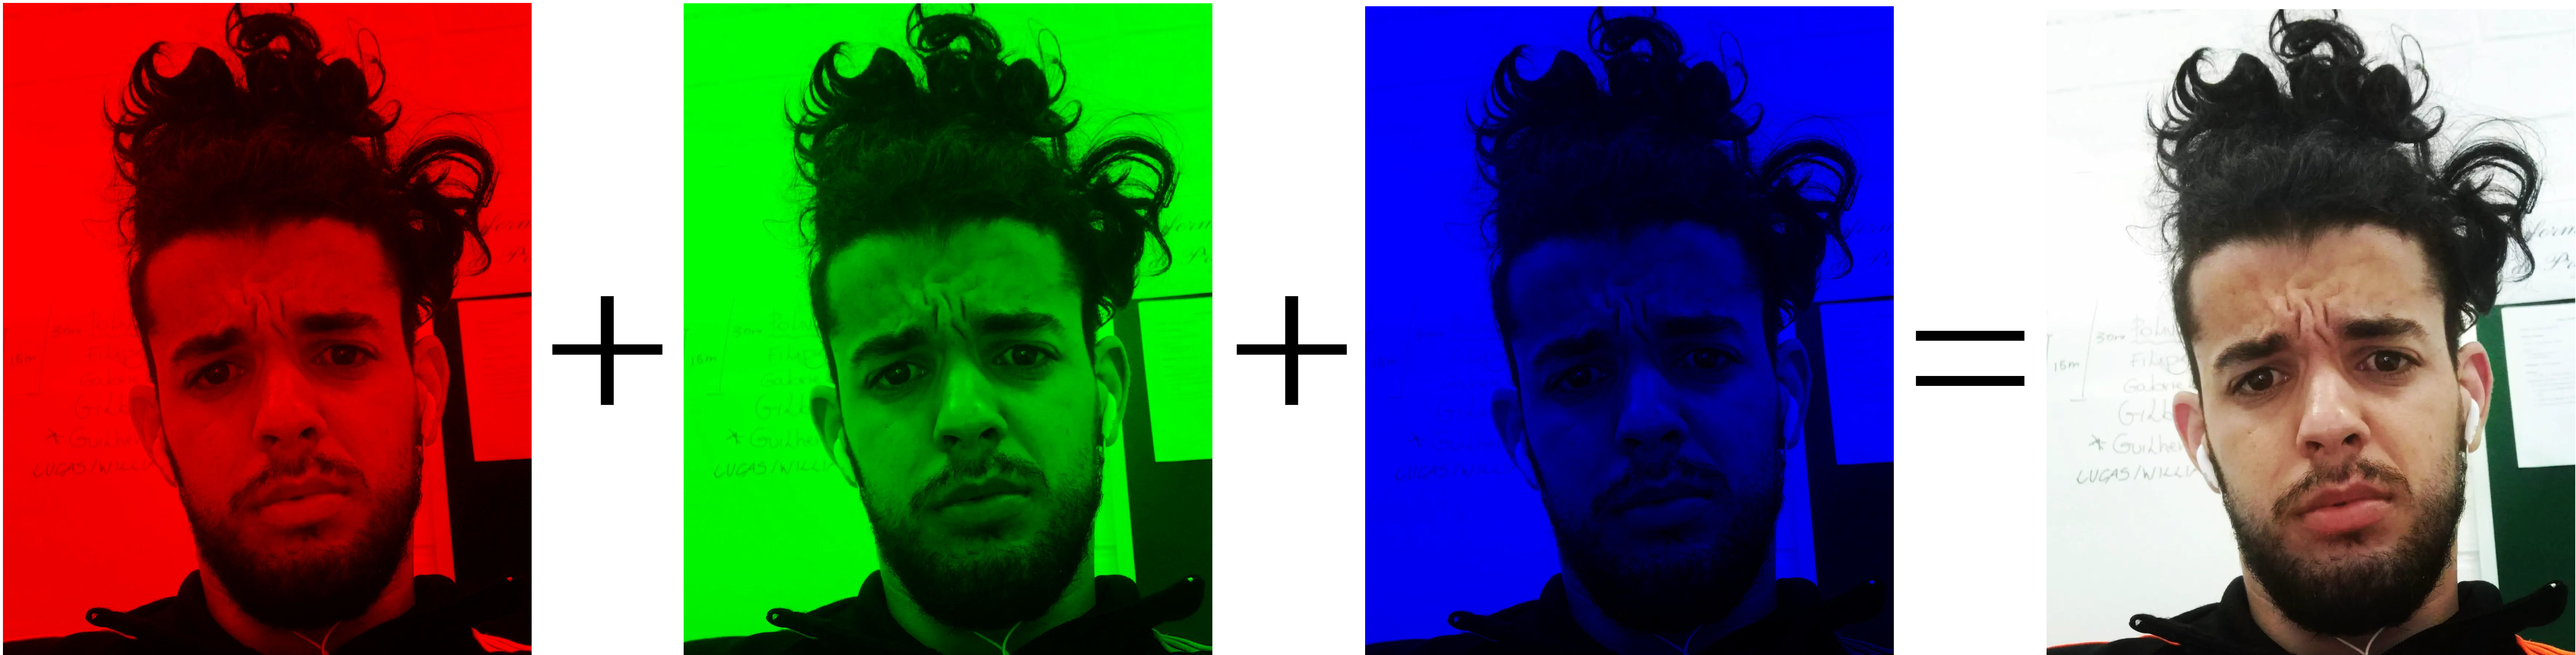
\includegraphics[scale=0.25]{figuras/Imagem_colorida/colored.png}
    \legend{Fonte: Elaborado pelo autor (2023).}
	\label{fig:Composicao de uma imagem RGB}
\end{figure}

Em uma imagem digital, a descrição da intensidade da luz pode ocorrer de maneiras distintas, relacionadas à natureza da imagem. A descrição da intensidade pode adotar valores binários representados por branco e preto e são frequentemente associados a conceitos como a presença ou a ausência de um objeto. Para  uma representação mais complexa de nuances de intensidade, texturas e detalhes é comum  que a intensidade da luz seja descrita em 8 bits ou seja 256 tonalidades diferentes de cores, variando de 0 a 255, onde 0 é preto e 255 é branco. Por fim para uma riqueza maior de detalhes é comum que imagens coloridas sejam descritas por uma tripla de canais \ac{RGB}  onde cada canal representa uma  cor, adotando valores de 8 bits por canal, portanto uma representação de 24 bits por pixel \cite{imagemIBM}.

\begin{figure}[!htb]
	\centering
	\caption{Representação de um pixel de uma imagem com três canais}
	\includegraphics[scale=1]{figuras/processamento_imagem/pixel.png}
    \legend{Fonte: \cite{imagemIBM}.}
	\label{fig:Representacao do Pixel de uma imagem com 3 canais}
\end{figure}



\subsection[Processamento de Imagem]{Processamento de Imagem}

O processamento de imagem refere-se à manipulação de imagens digitais para obter informações relevantes ou aprimorar a qualidade da imagem original por meio da aplicação de operações específicas. Em essência, o processamento de imagem atua como um tipo de processamento de sinais, onde a entrada é uma imagem digital e a saída resulta em uma nova representação da imagem ou informações derivadas dela. O objetivo central é extrair significado ou realçar características ao empregar uma série de técnicas e algoritmos, visando melhorar a utilidade ou interpretação das imagens \cite{imagemIBM}.

O processamento de imagens abrange um conjunto de etapas interligadas, cada uma contribuindo para transformar uma imagem digital em informações compreensíveis e relevantes. Inicialmente, ocorre a \aspas{aquisição de imagens}, onde os dados visuais são capturados por meio de câmeras, scanners ou sensores. Em seguida, passa-se pelo \aspas{pré-processamento}, onde a imagem é preparada para análise, eliminando ruídos e melhorando o contraste. A \aspas{segmentação} divide a imagem em regiões distintas, possibilitando focar em áreas específicas. A etapa de \aspas{representação e descrição} extrai características únicas de cada região, como texturas, formas e cores. Posteriormente, o \aspas{reconhecimento e interpretação} entra em cena, empregando algoritmos para identificar padrões, objetos ou informações relevantes com base nas características extraídas anteriormente. Esse processo cíclico de aquisição, pré-processamento, segmentação, representação e descrição, bem como reconhecimento e interpretação, forma o núcleo do processamento de imagens, permitindo a compreensão e análise de informações visuais de maneira mais eficaz e detalhada \cite{imagemMonocromatica}.


\begin{figure}[!htb]
	\centering
    \caption{Fluxograma das etapas do processamento de imagens digitais}
	\includegraphics[scale=0.4]{figuras/processamento_imagem/ProcessamentoImagem.png}
    \legend{Fonte: \cite{imagemMonocromatica}.}
	\label{fig:Fluxograma das etapas do processamento de imagens digitais}
\end{figure}




\subsection[Estimativa de pose humana]{Estimativa de pose humana}\label{sec:Estimativa de pose humana}
Identificação de Pose ou \ac{EPH} é um problema geral em Visão Computacional, que tem o objetivo de detectar a posição e a orientação de uma pessoa em imagens ou vídeos prevendo a localização de alguns pontos-chaves , conhecidos também como \textit{landmarks}, tais como  cabeça, ombros, cotovelos, mãos, quadril, joelhos e pés \cite{edh}.

\ac{EPH} pode ser bidimensional ou tridimensional, sendo o primeiro responsável por estimar as coordenadas X Y e o segundo as coordenadas X Y Z de um espaço virtual que geralmente é inferido a partir de uma imagem bidimensional. A \ac{EPH} pode também ser classificada de acordo com a quantidade de pessoas a serem estimadas podendo ser uma única pessoa ou de várias pessoas o que interfere nas resoluções possíveis pois a estimativa de postura de várias pessoas é ligeiramente mais difícil do que o caso de uma única pessoa \cite{edhDeep}.

\begin{figure}[!htb]
	\centering
    \caption{Captura de pontos de referência para estimativa de pose humana}
	\includegraphics[scale=0.2]{figuras/eph/keypoint.jpg}
    \legend{Fonte: \cite{tensorFlow_IMG}.}
	\label{fig:Captura de pontos de referencia para estimativa de pose humana}
\end{figure}





\subsection[Transformada de Hough]{Transformada de Hough}\label{sec:Transformada de Hough}


A Transformada de Hough é um algoritmo amplamente empregado na detecção de linhas retas em imagens. Sua utilidade é especialmente evidente ao buscar a extração de informações relacionadas a linhas presentes na imagem independentemente da orientação, localização ou continuidade. Em suma a Transformada de Hough opera transformando coordenadas cartesianas ($x$, $y$) da imagem em uma representação polar ($\rho$, $\theta$) no espaço de parâmetros, também conhecido como plano de Hough, esse plano é usado como um espaço de votação, onde é verificado quantos pontos compartilham uma mesma reta assim as retas que acumulam mais votos no espaço de votação são consideradas as retas detectadas na imagem \cite{transformadaHough1}.


Uma reta pode ser descrita como: $$y = mx + b$$

As características desta reta são a inclinação $m$ e a intersecção $b$ assim, uma reta $y = mx + b$ pode ser representada como um par ordenado $(b, m)$, porem em tal representação à medida em que a reta torna-se vertical, as magnitudes de $b$ e $m$ tendem ao infinito, contudo a mesma reta pode ser representada na forma:  $$\rho = x*cos(\theta)+y*sin(\theta)$$

Onde o parâmetro $\rho$ é a mínima distância da reta a origem, centro do plano, e $\theta$ é o ângulo de inclinação da normal à reta, sendo a normal uma linha perpendicular a direção da reta \cite{detectBar}.

\begin{figure}[!htb]
	\centering
    \caption{Representação da reta pelos parâmetros $\rho$ e $\theta$}
	\includegraphics[scale=2]{figuras/math/rhotheta.png}
    \legend{Fonte: \cite{parametrizacao}.}
    \label{fig:Representacao da reta pelos parametros}
\end{figure}

O plano de Hough é um plano bidimensional onde os eixos representam os parâmetros, sendo eixo $X$ representante do ângulo $\theta$ e o eixo $Y$ a representação da distância $\rho$ \cite{transformadaHough1}. Nesse contexto, um ponto no plano da imagem é atravessado por inúmeras retas, e a combinação de todas essas retas resulta na formação de uma curva senoidal no espaço de Hough \cite{detectBar}. Na figura \ref{fig:Representacao de um ponto no espaco parametrizavel}, o primeiro gráfico apresenta um ponto no plano. O segundo gráfico apresenta a representação desse ponto no espaço parametrizável $\rho$ e $\theta$.

\begin{figure}[!htb]
	\centering
    \caption{Representação de um ponto no espaço parametrizado por $\rho$ e $\theta$}
	\includegraphics[scale=0.5]{figuras/math/pontoEspacoParametrizavel.png}
    \legend{Fonte: \cite{parametrizacao}.}
	\label{fig:Representacao de um ponto no espaco parametrizavel}
\end{figure}

Dois pontos $p$ e $q$ no plano da imagem definem uma reta $pq$ e correspondem a duas senoides no plano de Hough. A interseção dessas duas senoides representa a reta $pq$ que passa pelos dois pontos no plano da imagem. Analogamente, 4 retas no plano da imagem correspondem a 4 senoides no plano de Hough que se acumulam em 4 pontos. Portanto, para realizar a detecção de uma reta, é necessário examinar as interseções das curvas senoidais. Isso é alcançado por meio da utilização de um acumulador, que consiste em uma lista destinada a armazenar todos os cruzamentos identificados. O processo de detecção de retas consiste em selecionar os cruzamentos que apresentam maior frequência na lista do acumulador \cite{transformadaHough2}. A figura \ref{fig:Representação da reta por meio do ponto de intersecção} apresenta, no primeiro gráfico, 8 pontos no plano pertencentes a duas retas. O segundo gráfico apresenta, no espaço parametrizável $\rho$ e $\theta$, 8 senoides que se interceptam em dois pontos diferentes. Assim, o local da interseção entre as senoides representa uma reta com parâmetros $\rho$ e $\theta$ específicos.


\begin{figure}[!htb]
	\centering
    \caption{Representação da reta por meio do ponto de intersecção}
	\includegraphics[scale=0.5]{figuras/math/senoidesIterseccao.png}
    \legend{Fonte: \cite{parametrizacao}.}
	\label{fig:Representacao da reta por meio do ponto de interseccao}
\end{figure}




\subsection[Detector de bordas de Canny]{Detector de bordas de Canny}\label{sec:Detector de bordas de Canny}

Um filtro de detecção de borda é um método utilizado no processamento de imagens para identificar mudanças abruptas na intensidade luminosa. Essas mudanças geralmente correspondem a limites entre diferentes objetos ou regiões na imagem. O filtro de detecção de borda realça essas mudanças, destacando os contornos e limites dos objetos presentes na imagem. Ele funciona calculando gradientes de intensidade em várias direções e destacando as regiões onde esses gradientes são mais acentuados. Em específico o filtro de Canny possui cinco etapas sendo elas: Redução de ruído; Cálculo de gradiente; Supressão não máxima; Limite duplo;Rastreamento de borda por histerese \cite{canny-edge-detection-python}.


\subsubsection[Redução de ruido]{Redução de ruido}
A redução de ruído ocorre com a aplicação de um filtro Gaussiano, uma técnica de convolução de imagens que, de acordo com um filtro, substitui o valor de cada pixel da imagem pela média da vizinhança. Isso tem como efeito a suavização da imagem, uma vez que as altas frequências que correspondem às transições abruptas são atenuadas \cite{filtroGaus}.

A convolução é uma operação matemática que combina duas funções para criar uma terceira. No contexto de processamento de imagens, a imagem original atua como uma das funções e o filtro (ou kernel) atua como a segunda função. O filtro é uma matriz de números que define como a vizinhança de cada pixel na imagem será ponderada e combinada para gerar o novo valor desse pixel na imagem resultante. O processo de convolução envolve a superposição do filtro sobre cada região da imagem e a multiplicação elemento a elemento dos valores do filtro com os valores correspondentes da imagem. Os resultados dessas multiplicações são somados para produzir o novo valor do pixel na imagem de saída \cite{convolucao}.

Kernel 5x5 utilizado no filtro Gaussiano \cite{kernel_gaus}:

\[
    \begin{bmatrix}
        1 & 4 & 7 & 4 & 1 \\
        4 & 16 & 26 & 16 & 4 \\
        7 & 26 & 41 & 26 & 7 \\
        4 & 16 & 26 & 16 & 4 \\
        1 & 4 & 7 & 4 & 1 \\
    \end{bmatrix}
\]

O tamanho do kernel está relacionado ao efeito de desfoque; quanto menor o kernel, menos visível é o desfoque. No filtro de Canny, é usado um kernel 5x5.




\subsubsection[Cálculo do Gradiente]{Cálculo do Gradiente}

As bordas correspondem a uma mudança na intensidade dos pixels. Portanto, o cálculo do gradiente em processamento de imagem refere-se à taxa de variação da intensidade luminosa em uma determinada região da imagem. Essa variação pode ser calculada usando operadores de detecção de borda na horizontal e vertical, ou seja, convolucionando a imagem com os respectivos kernels.

Filtro Sobel Horizontal:
\[
    \begin{bmatrix}
        -1 & 0 & 1 \\
        -2 & 0 & 2 \\
        -1 & 0 & 1 \\
    \end{bmatrix}
\]

Filtro Sobel Vertical:
\[
    \begin{bmatrix}
        1 & 2 & 1 \\
        0 & 0 & 0 \\
        -1 & -2 & -1 \\
    \end{bmatrix}
\]


Aplicando o filtro de Sobel na horizontal, tem-se $G_x$, que é o gradiente na direção horizontal. Aplicando o filtro de Sobel na vertical, tem-se $G_y$, que é o gradiente na direção vertical. Fazendo uso dessas informações, é possível chegar a $G_r$ com a fórmula:

$$G_R = \sqrt{G_x^2 + G_y^2}$$

$G_r$ refere-se ao valor resultante da combinação dos gradientes em duas direções (horizontal e vertical). Pontos onde $G_r$ é alto indicam mudanças bruscas de intensidade, muitas vezes correspondendo a bordas ou detalhes significativos na imagem. 

A inclinação $\theta$ que informa a direção do gradiente é calculado pela fórmula:
$$\theta(x, y) = \tan^{-1}\left(\frac{G_y}{G_x}\right)$$

Essa inclinação é perpendicular às arestas e arredondada para um dos quatro ângulos que representam as direções vertical, horizontal e duas diagonais.



\begin{figure}[!htb]
	\centering
    \caption{Imagem em preto e branco com filtro Gaussiano}
	\includegraphics[scale=0.25]{figuras/filter/sobel/f_normal.jpeg}
    \legend{Fonte: Elaborado pelo autor (2023)}
	\label{fig:Imagem em preto e branco com filtro de gaus}
\end{figure}

\begin{figure}[!htb]
	\centering
    \caption{Intensidade da mudança de gradiente usando operador de Sobel}
	\includegraphics[scale=0.25]{figuras/filter/sobel/f_sobel.jpeg}
    \legend{Fonte: Elaborado pelo autor (2023)}
	\label{fig:Intensidade da mudanca de gradiente}
\end{figure}



\subsubsection[Supressão não máxima]{Supressão não máxima}

É desejável que a imagem resultante apresente bordas precisas e nítidas. Para alcançar esse objetivo, aplica-se uma supressão não máxima, a fim de refinar as bordas detectadas. Nesse processo, o algoritmo percorre todos os pontos da matriz de intensidade de gradiente. Nos locais onde as bordas são encontradas, o algoritmo assegura que o pixel, que é um máximo local dentro de sua vizinhança na orientação do gradiente, seja mantido, e os que não são, sejam suprimidos \cite{canny-edge-detection-python}.

\begin{figure}[!ht]
	\centering
    \caption{Supressão não maxima}
	\includegraphics[scale=0.65]{figuras/filter/supressao_nao_maxima/supressao3.png}
    \legend{Fonte: \cite{canny-edge-detection-python}.}
	\label{fig:Supressao nao maxima}
\end{figure}

O procedimento do algoritmo é ilustrado na figura \ref{fig:Supressao nao maxima}, onde o pixel destacado em vermelho é aquele que está sendo processado. A linha em laranja representa a orientação do gradiente, ou seja, é uma linha perpendicular à borda. Os pixels de interesse presentes na vizinhança são destacados em azul, uma vez que estão na mesma orientação do gradiente. Se o valor do pixel realçado em vermelho for maior do que o valor dos pixels vizinhos destacados em azul, então esse pixel será mantido. Caso contrário, ele será suprimido, assegurando que somente os pontos mais significativos sejam preservados na representação das bordas \cite{canny-edge-detection-python}.


\subsubsection[Limite duplo]{Limite duplo}

O \aspas{limiar duplo} é uma técnica usada no processamento de imagens para segmentar uma imagem com base nos valores de intensidade dos pixels. Essa técnica envolve a definição de dois limiares diferentes, um limiar inferior $minVal$ e um limiar superior $maxVal$. Esses limiares dividem a escala de intensidade dos pixels em três intervalos: pixels abaixo de $minVal$, pixels entre $minVal$ e $maxVal$, e pixels acima de $maxVal$.

Com base nos limiares definidos, os pixels são classificados em três tipos:
Pixels abaixo de $minVal$ são desconsiderados, pois não possuem intensidade mínima para serem considerados relevantes.
Pixels entre $minVal$ e $maxVal$ são atribuídos à região de transição, na qual é necessária uma análise adicional.
Pixels acima de $maxVal$ são atribuídos à região de interesse, pois certamente contribuem para a borda final \cite{canny-edge-detection-python}.


\subsubsection[Limite de histerese]{Limite de histerese}
Baseado no limite duplo, o limite de histerese atua sobre os pixels que estão entre $minVal$ e $maxVal$, transformando pixels possivelmente relevantes em certamente relevantes se e somente se pelo menos um dos pixels ao redor daquele que está sendo processado for relevante, conforme descrito abaixo:

Os pixels que estão entre $minVal$ e $maxVal$ são classificados como bordas ou não-bordas com base em sua conectividade. Se estiverem conectados a pixels superiores a $maxVal$, serão considerados parte das bordas; caso contrário, serão descartados. Além das vizinhanças imediatas, verificações recursivas ou iterativas podem ser realizadas para explorar os pixels vizinhos dos pixels já marcados como relevantes. Isso permite estender a borda para pixels que não são diretamente vizinhos, mas que são alcançáveis por meio de pixels relevantes interligados \cite{opencv-canny}.




\subsection[Algoritmo de rastreamento ou Tracking]{Algoritmo de rastreamento ou Tracking}

O rastreamento, também conhecido como \textit{tracking}, pode ser conceituado como um conjunto de procedimentos computacionais elaborados com o propósito de monitorar e seguir o movimento ou a posição de objetos em uma sequência de imagens ao longo do tempo. Um algoritmo de rastreamento eficiente utiliza informações acumuladas sobre o objeto até o momento, com base no modelo de movimento do objeto que engloba sua posição, sua velocidade e direção do movimento, e também no modelo de aparência, que proporciona informações sobre a aparência específica do objeto com base nos quadros anteriores. Ou seja, enquanto a detecção de objetos ocorre em quadros de imagem isolados, o algoritmo de rastreamento é aplicado com base em uma sequência temporal, permitindo uma análise contínua do movimento do objeto \cite{tracking}.

O modelo de aparência desempenha um papel crucial no processo, permitindo a realização de uma busca precisa em uma pequena área próxima à localização prevista pelo modelo de movimento. Isso otimiza o processo de rastreamento, pois ocorre uma pesquisa local em vez de uma pesquisa global, garantindo a identidade do objeto. Mesmo com uma oclusão do objeto, é possível rastreá-lo, pois o rastreamento leva em consideração a localização e a aparência do objeto no quadro anterior. Entretanto, esse processo pode enfrentar desafios consideráveis, como a perda do objeto quando ele fica obstruído por um período prolongado ou quando sua velocidade é tão elevada que o algoritmo de rastreamento não consegue acompanhá-lo. Por isso, é comum que os algoritmos de rastreamento acumulem erros ao longo do tempo, comprometendo a precisão da localização do objeto. Para mitigar essas questões inerentes aos algoritmos de rastreamento, uma abordagem utilizada é executar periodicamente um algoritmo de detecção para identificação da nova posição do objeto e, em seguida, retransmitir essas informações para o rastreador, a fim de contribuir para a correção dos erros acumulados e manter um acompanhamento mais preciso do objeto ao longo do tempo \cite{tracking}.


Diversos algoritmos de rastreamento de objetos podem ser identificados, cada um com suas características particulares. Alguns exemplos notáveis incluem a Subtração de Plano de Fundo, o Casamento de Blocos, o \ac{SIFT} e o \ac{RANSAC}.

A Subtração de Plano de Fundo é capaz de identificar objetos destacando discrepâncias entre o plano de fundo e os objetos em movimento na cena. Por sua vez, o Casamento de Blocos realiza a comparação de blocos de pixels em diferentes quadros, o que lhe permite rastrear o movimento de objetos com eficácia. O algoritmo \ac{SIFT} desempenha um papel crucial ao extrair características distintivas de uma imagem, possibilitando o rastreamento robusto de objetos, mesmo diante de variações na escala, rotação ou iluminação. Finalmente, o \ac{RANSAC} é empregado para a estimativa de parâmetros de um modelo matemático previamente definido, de forma a se ajustar ao maior número possível de dados, ou seja, aqueles que são comumente chamados de \aspas{inliers}. Esses algoritmos oferecem soluções diversas e adaptáveis para a tarefa de rastreamento de objetos, cada um adequado a diferentes cenários e requisitos de aplicação \cite{tracking-algoritimo}.











\subsection[Pixelização]{Pixelização}

Quando uma imagem é ampliada ou exibida em uma resolução maior do que sua resolução original, os pixels individuais tornam-se visíveis, resultando em uma aparência granulada ou \aspas{pixelizada}, pois os detalhes da imagem original não podem ser representados com precisão em uma resolução mais baixa. Portanto, o filtro de pixelização resume-se em reduzir o número de valores de pixel distintos em uma imagem, substituindo um bloco quadrado de valores de pixel por seu valor médio \cite{pixelizacao}. 

\begin{figure}[htbp]
    \centering
    \caption{Imagem pixelizada com blocos de 32 x 32}
        \begin{minipage}{0.4\textwidth}
            \includegraphics[width=\textwidth]{figuras/pixelizacao/foto.jpeg}
        \end{minipage}
        \begin{minipage}{0.4\textwidth}
            \includegraphics[width=\textwidth]{figuras/pixelizacao/32.png}
        \end{minipage}
    \legend{Fonte: Elaborado pelo autor (2023)}
    \label{fig:Imagem pixelizada}
\end{figure}











\subsection[Limiarização]{Limiarização}

A limiarização, também conhecida como \textit{thresholding}, é uma técnica de processamento de imagem usada para classificar os pixels em uma imagem com base em um valor específico, denominado limiar. Isso resulta na categorização dos pixels em dois grupos distintos, geralmente sendo aqueles que têm valores acima do limiar e aqueles que têm valores abaixo ou iguais a ele. Esse método é amplamente utilizado em processamento de imagem para destacar ou segmentar objetos de interesse em relação ao restante da imagem \cite{limiarizacao}.

A limiarização pode ser empregada de duas maneiras distintas: ela pode transformar uma imagem em escala de cinza em uma imagem binarizada, tornando os pixels acima do limiar em branco e os pixels abaixo do limiar em preto. Alternativamente, ela pode ser utilizada para enfatizar uma faixa específica de frequência, convertendo apenas os pixels abaixo do limiar em preto ou apenas os pixels acima do limiar em branco \cite{opencv_thresholding}.


\section[Machine learning]{Machine learning}\label{sec:Machine learning}

Aprendizado de Máquina também conhecido como \ac{ML} é um ramo da \ac{IA} focado na análise de dados, que por meio de métodos estatísticos de aprendizado e otimização  permite computadores analisarem conjuntos de dados e identificar padrões e tendências históricas para prever modelos futuros \cite{ml}.

Comumente o algoritmo de aprendizado de máquina supervisionado consiste em três componentes: decisão, erro e otimização. 

O primeiro componente, decisão, é responsável por tomar decisões com base nas entradas fornecidas, que podem ser rotuladas ou não rotuladas. Esse componente é geralmente implementado como uma função matemática que mapeia as entradas para uma saída, seja uma classificação ou uma predição. Ele é responsável por transformar as entradas em informações úteis para o modelo, permitindo que o algoritmo aprenda a partir delas e tome decisões com base em novas entradas no futuro.

O segundo componente, erro, é responsável por avaliar a precisão da classificação ou da saída predita em relação à saída verdadeira, ou seja, os exemplos conhecidos. Esse componente é crucial porque permite uma analise do modelo.


O terceiro componente, otimização, é responsável por ajustar o modelo de modo que  minimize o  erro calculado pelo segundo componente e consequentemente seja possível melhorar a precisão da saída predita. 



\section[Autômatos Finitos]{Autômatos Finitos}


Os reconhecedores são sistemas formais conhecidos também como autômatos capazes de aceitar todas as sentenças que pertençam a uma determinada linguagem, rejeitando todas as demais. Por esse motivo, constituem uma forma alternativa às gramáticas para a representação finita de linguagens \cite{reconhecimento}.

Os reconhecedores apresentam quatro componentes fundamentais: uma memória (fita) contendo o texto de entrada do
reconhecedor, um cursor, que indica o próximo elemento da fita a ser processado, uma máquina de estados finitos, sem memória, e uma memória auxiliar opcional.


\begin{figure}[!htb]
	\centering
    \caption{Organização de um reconhecedor genérico}
	\includegraphics[scale=2]{figuras/AFD/reconhecedor.png}
    \legend{Fonte: \cite{AFD_reconhecedor}.}
	\label{fig:Organizacao de um reconhecedor generico}
\end{figure}


A fita de entrada é composta pela cadeia que o reconhecedor precisa analisar. Ela é dividida em células, cada uma contendo um único símbolo da sequência, que faz parte do alfabeto de entrada escolhido. A sequência é organizada da esquerda para a direita, começando pelo símbolo mais à esquerda na fita. O cursor, chamado normalmente de cabeçote de acesso, é utilizado para ler os símbolos da fita de entrada. Ele aponta sempre para o próximo símbolo que deve ser processado. Os movimentos do cursor são controlados pela máquina de estados, podendo ser unidirecionais (em geral, movendo-se apenas para a direita) ou bidirecionais (movendo-se tanto para a esquerda quanto para a direita), dependendo do tipo de reconhecedor \cite{reconhecimento}.

Alguns tipos de reconhecedores não apenas leem os símbolos da fita de entrada, mas também escrevem sobre a fita, substituindo os símbolos existentes por outros, de acordo com comandos definidos pela máquina de estados. A máquina de estados atua como o cérebro do reconhecedor, contendo um conjunto finito de estados que registram as informações coletadas e guiam o funcionamento do processo \cite{reconhecimento}.


Um \ac{AF} é um modelo abstrato e simplificado de um sistema computacional que pode ser usado para reconhecer padrões em sequências de símbolos \cite{afd}. Formalmente é representado como uma lista de cinco elementos  com : 
um conjunto finito de estados representado por $Q$, um alfabeto de entrada representado por $\Sigma$, Funções de transição representada por $\delta : Q \times \Sigma \rightarrow Q$, estado inicial $q_0 \in Q$ e um conjunto de estados finais $F \subseteq Q$ portanto um autômato finito é representado como uma 5-upla $(Q, \Sigma, \delta, q_0, F)$

Sendo que o estado é uma representação de uma condição específica em que o autômato pode se encontrar durante a sua execução, o alfabeto é o conjunto finito de símbolos que o autômato pode receber como entrada, e as funções de transição definem como o autômato muda de um estado para outro em resposta a um símbolo de entrada.

As funções de transição são denotadas como $\delta(e_0, 1) = e_1$, em outras palavras, essa regra específica indica que um autômato no estado $e_0$, ao ler o caractere 1, se move para o estado $e_1$.

Também é possível representar um \ac{AF} de modo mais visual por meio de um diagrama de estados onde é ilustrado os estados do autômato, suas transições e os símbolos de entrada. Cada estado é representado por um círculo e as transições são indicadas por setas entre esses círculos, rotuladas com os símbolos de entrada correspondentes \cite{afd}.

Em um diagrama de estados, cada estado é representado por um círculo, enquanto as transições são marcadas por setas que conectam esses círculos. Essas setas são rotuladas com os símbolos de entradas correspondentes. O estado inicial é indicado com uma seta apontando para ele, originada de um ponto vazio. Os estados de aceitação são ilustrados por círculos duplos.

Portanto um \ac{AF} chamado $M_1$ que aceita qualquer número binário impar pode ser representado de 2 maneiras,  por uma 5-upla ou um diagrama de estados:

\begin{itemize}
    \item[$M_1$] = $(Q, \Sigma, \delta, q_1, F)$, onde:
    \item[$Q$] = $\{q_1, q_2, q_3\}$
    \item[$\Sigma$] = \{0, 1\}
    \item [$\delta$] é descrito como
    \item [ ]
        \begin{tabular}{c|cc}
            & 0 & 1 \\ \hline
            $q_1$ & $q_1$ & $q_2$ \\
            $q_2$ & $q_3$ & $q_2$ \\
            $q_3$ & $q_2$ & $q_2$ \\
        \end{tabular}
    \item[$q_1$] é o estado inicial
    \item[$F$] = \{$q_2$\}
\end{itemize}

\begin{figure}[!htb]
	\centering
    \caption{Diagrama de estados de $M_1$}
	\includegraphics[scale=1]{figuras/AFD/m1.png}
    \legend{Fonte: \cite{AFD_M1}.}
	\label{fig:Diagrama de estados}
\end{figure}

Um reconhecedor e um \ac{AF} são conceitos relacionados, mas cada um tem um papel específico sendo esse um modelo abstrato e aquele um sistema ou algoritmo que é capaz de identificar ou detectar algo em um conjunto de dados.

% ----------------------------------------------------------
\chapter{Tecnologias e Métodos}
% ----------------------------------------------------------
Neste capítulo são apresentadas as metodologias adotadas, juntamente com as ferramentas, bibliotecas e bases de dados que foram utilizadas no desenvolvimento desse trabalho.

Em Materiais \ref{sec:Materiais} são apresentados as ferramentas utilizadas, como: linguagem de programação, bibliotecas utilizadas e as especificações técnicas do sistema computacional utilizado. Na seção de Método \ref{sec:Metodo} é descrito os passos do desenvolvimento a serem tomados para a reprodução deste trabalho, para que ao final seja possível executar os experimentos e verificar os resultados obtidos.


\section[Materiais]{Materiais}\label{sec:Materiais}

Para o desenvolvimento deste trabalho foi necessário o uso  de linguagens de programação e bibliotecas, abaixo segue uma lista com as ferramentas  utilizadas:

\begin{itemize}




   \item Python: Idealizada e desenvolvida no início dos anos 90,  com o objetivo de otimizar a leitura de códigos, Python, é uma linguagem de programação de alto nível, dinâmica, interpretada, modular, multiplataforma e orientada a objetos com uma sintaxe simples e facilmente intercambiável com outras linguagens e com uma grande coleção de bibliotecas \cite{python}. Foi utilizado o python na versão 3.8.10.

   \item Open Source Computer Vision Library: Originalmente, desenvolvida pela Intel no ano de 2000, o openCV como tambem é conhecido é  uma biblioteca multiplataforma, totalmente livre ao uso acadêmico e comercial, para o desenvolvimento de aplicativos na área de Visão computacional com interfaces em C++, Python, Java e MATLAB \cite{openCV} Foi utilizado OpenCV na versão v4.7.0.
   
   \item MediaPipe: A MediaPipe é um projeto de código aberto desenvolvido pela Google, apresentando um conjunto de recursos e módulos pré-construídos, desenvolvidos com base no TensorFlow Lite. Esse framework destina-se a facilitar a implementação de técnicas de \ac{IA} e \ac{ML} em diversos ambientes, com foco na análise de mídia em tempo real e streaming contínuo. A característica distintiva da MediaPipe reside na execução integral do processamento dos dados de entrada diretamente no dispositivo, permitindo sua aplicação prática em uma ampla gama de plataformas, incluindo dispositivos móveis (Android, iOS), ambientes web, sistemas de desktop, dispositivos de borda e Internet das Coisas (IoT)\cite{mediapipe} Foi utilizada a versão v0.9.2.1 que é baseado em modelos ja treinados e usa uma cadeia de operações para prever pontos de referência de pose. O primeiro modelo detecta a presença de corpos humanos dentro de um quadro de imagem, e o segundo modelo localiza até 33 pontos de referência nos corpos \cite{mediapipe_pose_landmarker} que representam a localização aproximada das seguintes partes do corpo:


\begin{figure}[!htb]
	\centering
	\includegraphics[scale=0.3]{figuras/eph/pose_landmarks.png}
	\caption{Pontos de referência}
	\label{fig:Pontos de referencia}
\end{figure}

\begin{itemize}
    \item[0] - nariz
    \item[1] - olho esquerdo (interno)
    \item[2] - olho esquerdo
    \item[3] - olho esquerdo (externo)
    \item[4] - olho direito (interno)
    \item[5] - olho direito
    \item[6] - olho direito (externo)
    \item[7] - orelha esquerda
    \item[8] - orelha direita
    \item[9] - boca (esquerda)
    \item[10] - boca (direita)
    \item[11] - ombro esquerdo
    \item[12] - ombro direito
    \item[13] - cotovelo esquerdo
    \item[14] - cotovelo direito
    \item[15] - pulso esquerdo
    \item[16] - pulso direito
    \item[17] - mindinho esquerdo
    \item[18] - mindinho direito
    \item[19] - indicador esquerdo
    \item[20] - indicador direito
    \item[21] - polegar esquerdo
    \item[22] - polegar direito
    \item[23] - quadril esquerdo
    \item[24] - quadril direito
    \item[25] - joelho esquerdo
    \item[26] - joelho direito
    \item[27] - tornozelo esquerdo
    \item[28] - tornozelo direito
    \item[29] - calcanhar esquerdo
    \item[30] - calcanhar direito
    \item[31] - dedo do pé esquerdo (indicador)
    \item[32] - dedo do pé direito (indicador)
\end{itemize}\label{lst:Pontos de referencia}

    \item GitHub: O GitHub é uma plataforma de hospedagem em nuvem, lançada em 10 de abril de 2008 originalmente desenvolvida pela GitHub Inc e atualmente mantida pela Microsoft Corporation. Essa plataforma faz uso do Git um sistemas de controle de versão que mantém um registro abrangente e detalhado de todas as alterações realizadas no código-base, permitindo um rastreamento preciso do histórico de mudanças e do progresso do desenvolvimento ao longo do tempo. Sua capacidade de facilitar a colaboração eficaz e de manter um histórico completo. Alem de desempenhar um papel essencial na colaboração entre desenvolvedores, proporcionando um ambiente colaborativo para projetos compartilhados\cite{github}.

 \end{itemize}

Na busca por uma abordagem robusta e fundamentada para a analise quantitativa do uso de memoria, e tempo de execução, é imperativo descrever os materiais empregados na realização deste estudo e detalhar as caracteristicas dos principais componentes relevantes para o desempenho durante o procesamento da imagem, abaixo segue uma lista com as caracteristicas:

\begin{itemize}

\item Notebook IdeaPad 3 82MF0004BR AMD Ryzen 7 5700U 15,6" 8GB 

\item Pocessador
\subitem CPU: AMD Ryzen 7 5700U with Radeon Graphics
\subitem Frequência de clock: 1400 MHz
\subitem Número de núcleos: 16
\subitem Thread(s) per núcleo: 2

\item Memória (RAM)
\subitem Tipo: DDR4
\subitem Capacidade: 8 GB
\subitem Frequencia: 1600 Mhz

\item Placa de video
\subitem Nome: AMD Radeon RX Vega 8 Graphics
\subitem Driver em Uso: amdgpu
\subitem Capacidade de memória VRAM: 2.09 GB

\item Memoria (SSD)
\subitem Capacidade de armazenamento: 256 GB
\subitem Destinado a swap: 50 GB
\subitem Interface: M2
\subitem Protocolo: NVMe

\item Sistema operacional GNU/Linux
\subitem Distribuição: Linux Mint 20.2
\subitem Kernel: 5.15.0-76-generic
\subitem LSB Version: core-11.1.0ubuntu2-noarch:printing-11.1.0ubuntu2-noarch:security-11.1.0ubuntu2-noarch




\end{itemize}


\section[Método]{Método}\label{sec:Metodo}


No desenvolvimento deste trabalho, adotou-se uma abordagem que combina elementos do processo padrão de elaboração de trabalhos acadêmicos com a estruturação das etapas de um sistema de visão computacional, conforme documentado na literatura \cite{imagemMonocromatica}.  Essa abordagem foi escolhida para o desenvolvimento de um artefato em nível de prova de conceito, envolvendo os conteúdos abordados, o que torna este trabalho uma contribuição original e prática para a área em questão. Portanto, foram realizadas as seguintes etapas:


 \begin{itemize}
   \item Realização de revisão da literatura abordando o uso de visão computacional associado ao treinamento físico.
   \item Escolha da linguagem de programação para desenvolvimento da ferramenta.
   \item Escolha das tecnologias para realização do processamento de imagem.
   \item Escolha da ferramenta utilizada para a detecção de pose humana.  
   %\item Realização de revisão da literatura abordando conceitos como insuficiencia muscular.
   \item Realização de revisão da literatura abordando a importancia do movimento excentrico para o ganho de força
   %\item Realização de revisão da literatura abordando o grau de amplitude de movimento do bíceps braquial.
   \item Criação de uma estrategia para deteção do movimento correto de barra fixa    
   %\item Analise do movimento de barra fixa focando no tempo de contração excentrica,concentrica e isometrica.
   %\item Analise da amplitude de movimento de flexao associada a ativação do biceps braquial
   \item Desenvolvimento de uma Ferramenta computacional para detecção da execução correta da barra fixa.
   \item Avaliação dos resultados.
   
 \end{itemize}

 A ferramenta desenvolvida atua apartir de uma gravação no plano coronal da execução do movimento de barra fixa processando a imagem de modo a detectar a barra e os pontos de referêcia do corpo humano e logo em seguida ocorre a segmentação da imagem e calculos algébricos retornando o estado atual do movimento de barra fixa e dados sobre o movimento como forma de feedback sobre o movimento. Todo este processo segue o fluxograma abaixo.

\begin{figure}[!htb]
	\centering
	\includegraphics[scale=0.7]{figuras/diagrama/processo.png}
	\caption{fluxograma}
	\label{fig:fluxo}
\end{figure}






\chapter{Projeto e Desenvolvimento}
Nesta seção são detalhados os passos e decisões tomadas ao decorrer do desenvolvimento deste trabalho. São apresentadas as etapas de implementação e integração com outras soluções utilizadas, assim como a execução e comparação dos resultados obtidos.

\section[Uso de visão computacional associado ao treinamento físico]{Uso de visão computacional associado ao treinamento físico}\label{sec:Uso de visao computacional associado ao treinamento fisico}

Foi feita uma revisão bibliografica com objetivo de encontrar ferramentas ou trabalhos disponíveis que associam a visão computacional a algum tipo de atividade física, portanto foram formuladas algumas questões de pesquisa para identificar trabalhos pertinentes que possam agregar a este trabalho de alguma forma, são elas:
 \begin{itemize}
   \item Q1: Em quais atividades físicas foi utilizada a visão computacional como ferramenta?
   \item Q2: Como a visão computacional foi empregada em determinada atividade física?
   \item Q3: Quais métricas ou parâmetros são frequentemente extraídos das imagens
 \end{itemize}

No decorrer desta revisão, foram identificados diversos estudos relevantes na área, com destaque especial para o trabalho intitulado \aspas{Análise postural digital para ciclistas} \cite{vcBicicleta}. Um dos objetivos desse estudo foi o desenvolvimento de um sistema digital denominado BFit4All. Esse sistema tem como objetivo identificar e propor ajustes na bicicleta com base nas análises posturais de ciclistas durante a atividade de pedalar por meio de fotografias. É importante ressaltar que a abordagem adotada nesse trabalho para a segmentação da imagem digital faz uso de marcadores fixados ao corpo do ciclista para destacar os pontos de referência e assim calcular as angulações entre eles. Embora essa metodologia revele-se eficaz em diversos aspectos, é válido destacar que esta implementação requer uma intervenção prévia à captura do vídeo.

Também foram identificados outros trabalhos relevantes, como os de Pádua (\citeyear{vcFutebol}) e Paulichen (\citeyear{futebolTatica}). Esses estudos abordam o desenvolvimento de sistemas de visão computacional que utilizam algoritmos de rastreamento de objetos. Tais sistemas extraem informações detalhadas sobre o posicionamento, trajetória, velocidades e distâncias percorridas pelos jogadores de futsal. As informações resultantes desse processo proporcionam indicadores de natureza tática e fisiológica, que se mostram valiosos para a equipe técnica. Uma abordagem interessante que foi adotada no trabalho de Paulichen para o rastreamento de uma área de interesse foi a aplicação do filtro de Kalman, uma técnica de estimativa e previsão que combina informações medidas e modelos matemáticos para melhorar a precisão de uma estimativa, reduzindo o ruído e as incertezas nas medições.

Em relação às ferramentas computacionais para análise e aprimoramento do treinamento, é interessante destacar a referência ao Dartfish feita no trabalho de Franke (\citeyear{vcBicicleta}). O Dartfish é uma plataforma amplamente adotada por treinadores, atletas e equipes esportivas, e seu destaque é reforçado pelo fato de ter sido utilizado por 73\% dos medalhistas olímpicos em Pequim. Essa plataforma de software comercial oferece uma abordagem abrangente para a otimização do desempenho esportivo por meio da análise de vídeo. Sua capacidade de rastrear objetos e movimentos em vídeos permite uma análise minuciosa e direcionada a elementos específicos. Ao segmentar e examinar detalhadamente o posicionamento, trajetória e dinâmica dos movimentos dos atletas, o Dartfish proporciona insights valiosos facilitando a identificação de padrões, embasamento de decisões e implementação de ajustes táticos e técnicos com base em informações visuais concretas \cite{dartfish}. Embora essa plataforma seja uma das mais conceituadas soluções de análise de vídeo para desempenho esportivo, vale destacar que ela é intimamente dependente de um profissional qualificado para analisar e assessorar o treinamento esportivo.



\section[Escolha da linguagem de programação para desenvolvimento da ferramenta]{Escolha da linguagem de programação para desenvolvimento da ferramenta}\label{sec:Escolha da linguagem de programacao para desenvolvimento da ferramenta}

A escolha da linguagem de programação para a implementação deste projeto foi baseada nos requisitos do sistema proposto. Dentre as opções consideradas, JavaScript e Python, optou-se pelo uso da linguagem Python em sua versão 3.8.10 devido a uma série de fatores que se alinham de forma ideal com os objetivos deste trabalho, sendo eles:

A facilidade de manutenção do código ao longo do ciclo de vida do sistema, pois uma linguagem de programação com uma sintaxe clara e legível é particularmente vantajosa para a produção de um código facilmente compreensível, facilitando significativamente as atividades de manutenção contínua e de depuração. Um aspecto que se torna crucial na busca pela robustez e estabilidade do sistema ao longo do tempo \cite{clean_code}.

Agregou à escolha o fato da linguagem escolhida ter uma ampla biblioteca padrão e um vasto ecossistema de pacotes de terceiros que permitem a manipulação de imagens.

Dessa forma, a escolha do Python reflete diretamente na minimização dos desafios associados à evolução e manutenção do código-fonte, contribuindo para um desenvolvimento mais fluido e eficaz do projeto focado na produtividade.



\section[Escolha da biblioteca para realização do processamento de imagem]{Escolha da biblioteca para realização do processamento de imagem}\label{sec:Escolha da biblioteca para realizacao do processamento de imagem}

Nesta seção do trabalho, será abordado o processo de escolha das bibliotecas, levando em consideração os critérios relevantes para assegurar a eficácia e o desempenho na manipulação de imagens.

\subsection{Open Source Computer Vision Library}
Para a realização do processamento de imagem, a escolha recaiu sobre a biblioteca \ac{openCV}. A decisão de adotá-la foi primordialmente embasada na sua perfeita integração com a linguagem selecionada, Python.

A sólida reputação do \ac{openCV} na indústria, usado por empresas de renome como a Microsoft, Google e Intel, entre outras, torna-o uma escolha altamente relevante. Além disso, sua proeminente utilização no meio acadêmico oferece uma perspectiva valiosa de compartilhamento de conhecimento e habilidades para futuros projetos e oportunidades \cite{opencv_docs}. 

A extensa documentação disponível, juntamente com uma extensa comunidade engajada e ativa, simplificam tanto a compreensão quanto a implementação. Assim, a escolha do \ac{openCV} como biblioteca para o processamento de imagem é respaldada pelo potencial de eficiência e facilidade de implementação que essa escolha oferece \cite{opencv_docs}.

Por fim, e um dos mais importantes aspectos levados em consideração, foi a eficácia e o desempenho do \ac{openCV} que é escrito em C++ e otimizado para aproveitar recursos de hardware, o que resulta em alto desempenho e eficiência no processamento de imagens.

\subsection{MediaPipe}

Dentro do contexto do processamento de imagem, optou-se por empregar a biblioteca MediaPipe para a detecção de poses. A decisão de incorporá-la foi fortemente motivada pela sua perfeita integração com a linguagem Python, destacando-se assim como uma alternativa coesa.

Vale ressaltar que a biblioteca MediaPipe é voltada para a simplificação da implementação de técnicas de \ac{IA} e \ac{ML} em diversos cenários, com um enfoque específico na análise de mídia. Seu diferencial reside na disponibilidade de modelos pré-treinados e customizáveis, permitindo uma integração eficaz e adaptável ao projeto em questão \cite{mediapipe_guide}.

Por atuar com uma aplicação de \ac{IA} e \ac{ML} que trabalha com modelos ja treinados, o processamento dos dados de entrada ocorre completamente no dispositivo o que foi um ponto relevante, garantindo a persistência e funcionalidade contínua da ferramenta desenvolvida, independentemente da ação do tempo em relação a disponibilidade de servidores externos.

Outro ponto relevante para a escolha dessa ferramenta foi o fato de que ela se destaca pela capacidade de fornecer resultados precisos e reais na detecção de poses, o que possibilita a emissão de um feedback por parte da ferramenta desenvolvida.




\section[Estratégia para detecção do movimento correto de barra fixa]{Estratégia para detecção do movimento correto de barra fixa}\label{sec:Estrategia para deteccao do movimento correto de barra fixa}


Esta seção delineia a estratégia utilizada para detectar o movimento correto da barra fixa na ferramenta desenvolvida. O movimento de barra fixa se desdobra em um padrão que segue etapas distintas, as quais podem ser divididas em três fases bem definidas.

A primeira etapa engloba a posição inicial, onde o praticante se encontra pendurado na barra em pegada pronada, com os cotovelos estendidos e sem que os pés façam contato com o solo. A segunda etapa engloba a fase de contração concêntrica, onde o indivíduo eleva seu corpo até que seu queixo ultrapasse o nível da barra, sem fazer movimentos de quadris ou pernas e com extensão da coluna cervical como forma de auxílio na execução do movimento. Por fim, a terceira etapa engloba a fase de contração excêntrica, que envolve o retorno do corpo à posição inicial após a ultrapassagem da barra. Cabe salientar que a meta é fazer com que o queixo ultrapasse a barra independentemente de se manter assim por muito ou pouco tempo. Portanto, é possível adicionar mais uma fase, totalizando quatro, mas a essência do movimento se dá em três fases.

Dessa forma, optou-se por adotar a ideia de um reconhecedor para analisar o movimento de barra fixa. Nesse contexto, a fita é representada por um vídeo, no qual cada quadro do vídeo, comumente chamado de \textit{frame}, representa uma célula da fita. Os \textit{frames} são submetidos a um processamento afim de extrair informações cruciais que serão usadas na máquina como um caractere presente na fita. Para conduzir essa análise, é usada a ideia de uma máquina com cursor fixo que desloca a fita de maneira linear para a esquerda, lendo sequencialmente os caracteres presentes à direita. Além disso, essa abordagem incorpora uma memória auxiliar, responsável por registrar as transições entre dois estados específicos. Tal estratégia é implementada visando a precisão na contabilização dos movimentos corretos realizados durante o teste, conferindo, assim, uma avaliação meticulosa e sistemática do movimento de barra fixa.

Em suma, foi elaborado um \ac{AFD} que inicia em um estado de preparação e avança para o estado de início somente quando as mãos estão na barra e os braços estão esticados.

O movimento concêntrico ocorre quando, partindo do estado inicial, os braços deixam de estar esticados e se mantêm nessa posição até que a meta seja alcançada ou ocorra um movimento ilegal dos quadris.

O movimento de barra é contabilizado no momento em que o \ac{AFD} transita do estado concêntrico para o estado de meta. O estado de meta permanece enquanto o queixo estiver sobre a barra.

O movimento excêntrico começa quando, a partir do estado de meta, o queixo deixa de estar sobre a barra. É importante salientar que, como a meta foi atingida, os movimentos das pernas nesse momento não influenciam na contabilização dos movimentos de barra fixa. No entanto, mesmo não sendo contados, não deixa de ser um movimento indesejado. O movimento excêntrico se mantém até que o executor retorne à posição inicial.

A qualquer momento em que o executor retirar a mão da barra, o teste é automaticamente encerrado, levando o \ac{AFD} ao estado Fim.

O \ac{AFD} construído opera em relação a um alfabeto específico. Esse alfabeto é constituído por características extraídas de cada \textit{frame}. Cada símbolo do alfabeto é representado por uma 4-upla de características (A, B, C, D). Sendo as características explicadas a seguir.

\begin{itemize}
    \item[A] Presença das mãos na barra.
    \item[B] Ocorrência da extensão dos cotovelos.
    \item[C] Ocorrência da ultrapassagem do queixo sobre a barra.
    \item[D] Existência de movimento nos quadris.
\end{itemize} 

Cada elemento da 4-upla pode receber um valor binário, sendo 0 para representar a ausência ou 1 para representar a existência de tal característica em um determinado \textit{frame}. Portanto, o alfabeto do \ac{AFD} pode ser representado da seguinte forma:

\[
\begin{aligned}
\Sigma = \{ &(0, 0, 0, 0), (0, 0, 0, 1), (0, 0, 1, 0), (0, 0, 1, 1), \\
            &(0, 1, 0, 0), (0, 1, 0, 1), (0, 1, 1, 0), (0, 1, 1, 1), \\
            &(1, 0, 0, 0), (1, 0, 0, 1), (1, 0, 1, 0), (1, 0, 1, 1), \\
            &(1, 1, 0, 0), (1, 1, 0, 1), (1, 1, 1, 0), (1, 1, 1, 1) \}
\end{aligned}
\]

O \ac{AFD} desenvolvido consiste em um conjunto de sete estados:
\[
\begin{aligned}
\{ &\text{Preparação, Início, Concêntrica, Meta, Excêntrica, Erro, Fim} \}
\end{aligned}
\]
O estado \aspas{Preparação} é o estado inícial do \ac{AFD} representado qualquer momento que antecede o começo do teste de barra fixa como um todo. Um exemplo disso são os momentos que o executor se aproxima da barra fixa e se prepara para assumir a posição inicial.

O estado \aspas{Início} simboliza o começo do movimento da barra fixa. Nesse ponto, o executor deve estar pendurado na barra com a pegada pronada, cotovelos estendidos e sem contato dos pés com o solo.

O estado \aspas{Concêntrica} simboliza a transição da posição inicial até a realização da meta, que é a ultrapassagem do queixo sobre a barra. Esse estado tem o nome de concêntrica, pois, para o alcance da meta, é necessário que o executor recrute as fibras musculares dos membros superiores, realizando uma contração concêntrica afim de alcançar a meta.

O estado \aspas{Meta} simboliza a realização da meta, ou seja, houve a ultrapassagem do queixo sobre a barra.

O estado \aspas{Excêntrica} simboliza a transição de volta à posição inicial, ou seja, pendurado na barra com a pegada pronada, cotovelos estendidos e sem contato dos pés com o solo. Esse estado tem o nome de excêntrica, pois, para voltar à posição inicial, é necessário que o executor realize uma contração excêntrica até o momento em que os cotovelos fiquem totalmente esticados.

O estado \aspas{Erro} representa todas as instâncias em que o teste está em andamento, mas devido a uma falha do executor, parâmetros são identificados que exigem um retorno à posição inicial para que o movimento seja considerado correto. Por exemplo, isso pode ocorrer quando o executor realiza um movimento de balanço com o quadril para facilitar a execução do movimento. Em outras palavras, se o executor alcança a meta de ultrapassar o queixo acima da barra, mas utiliza o impulso das pernas para isso, o movimento não será considerado válido. Portanto, é necessário retornar à posição inicial e reiniciar o movimento. 

Por último, o estado \aspas{Fim} representa o momento em que o teste é encerrado e os movimentos não são mais contabilizados.

Portanto, o conjunto de estados finais do \ac{AFD} pode ser representado da seguinte forma: $F=\{Fim\}$

As funções de transições estão representadas no diagrama de estados a seguir:

\begin{figure}[H]
	\centering
	\caption{Diagrama de Estados do AFD desenvolvido}
	\includegraphics[scale=0.4]{figuras/AFD/afd_barra.png}
    \legend{Fonte: Elaborado pelo autor (2023)}
	\label{fig:transicaoAFD}
\end{figure}


\section[Extração de informação frame a frame]{Extração de informação frame a frame}\label{sec:Extracao de informacao frame a frame}

Dentro do processamento de imagem, a segmentação é a etapa onde a imagem é dividida em regiões ou componentes significativos que podem ser analisados e processados de forma independente. Em outras palavras, a segmentação visa identificar áreas distintas na imagem que correspondem a objetos, padrões, bordas ou características de interesse \cite{imagemMonocromatica}.

O objetivo da ferramenta é operar em um ambiente controlado. Entretanto, devido às características específicas da infraestrutura do local de teste, tornou-se essencial incorporar uma máscara para uma manipulação adequada de cada quadro. Com esse propósito, uma máscara previamente elaborada a partir do primeiro quadro do vídeo foi aplicada, utilizando a função bitwise\_and, disponibilizada na biblioteca \ac{openCV}. A operação bitwise\_and consiste em um processo de AND bit a bit entre os valores dos pixels do quadro e os valores correspondentes da máscara. O resultado é uma nova imagem em que os pixels que não fazem parte das regiões brancas da máscara são convertidos para preto, enquanto os pixels que pertencem a essas regiões permanecem intactos. A finalidade dessa máscara é realçar a região de interesse dentro do quadro, permitindo um foco preciso durante a etapa de segmentação da imagem.
\begin{figure}[htb]
    \centering
    \caption{Ambiente de gravação e Mascara Preto e Branca criada apartir do mesmo}
        \begin{minipage}{0.4\textwidth}
            \includegraphics[width=\textwidth]{figuras/filter/mask/ambiente.png}
        \end{minipage}
        \begin{minipage}{0.4\textwidth}
            \includegraphics[width=\textwidth]{figuras/filter/mask/mask.png}
        \end{minipage}
    \legend{Fonte: Elaborado pelo autor (2023)}
    \label{fig:maskAmbiente}
\end{figure}

\subsection[Detecção da barra]{Detecção da barra}\label{sec:Deteccao da barra}

Para a detecção da barra fixa, foi empregado o filtro de Canny \ref{sec:Detector de bordas de Canny} com o intuito de mitigar ruídos e enfatizar as bordas proeminentes. Para essa finalidade, foi adotada a função incorporada à biblioteca \ac{openCV}, sendo parametrizada da seguinte forma: o limite inferior do processo de histerese foi estabelecido em 50, o limite superior definido em 100, e o tamanho do kernel aplicado ao operador Sobel foi estipulado como 3. 

Após a etapa de pré-processamento da imagem, foi empregada a Transformada de Hough \ref{sec:Transformada de Hough}, também disponibilizada na biblioteca \ac{openCV}. Essa aplicação foi configurada com os seguintes parâmetros: a resolução da distância no acumulador, em pixels, foi definida como 1; a resolução angular no acumulador, em radianos, foi estabelecida em $\pi$/180, equivalente a 1 grau; e o limiar do acumulador foi fixado em 150. Essas configurações asseguram a avaliação de cada pixel para sua inclusão ou não como parte de uma reta, além de garantir uma inclinação mínima de 1º de uma reta a outra e que sejam consideradas retas apenas aquelas que tiverem 150 votos ou mais contabilizados no acumulador.

\begin{figure}[htb]
    \centering
        \caption{Aplicação do filtro de Canny.}
        \begin{minipage}{0.45\textwidth}
            \includegraphics[width=\textwidth]{figuras/filter/canny/mask.png}
        \end{minipage}
        \begin{minipage}{0.45\textwidth}
            \includegraphics[width=\textwidth]{figuras/filter/canny/canny.png}
        \end{minipage}
    \legend{Fonte: Elaborado pelo autor (2023)}
    \label{fig:maskCanny}
\end{figure}

O resultado da Transformada de Hough \ref{sec:Transformada de Hough} foi filtrado, selecionando apenas retas horizontais com uma tolerância de 10°, ou seja, somente retas cujo valor absoluto do ângulo é menor que o valor da tolerância, ou ainda, cujo valor absoluto da diferença entre 180 e a tolerância é menor que o valor absoluto do ângulo.

Após a etapa inicial de filtragem, uma segunda filtragem foi aplicada para selecionar exclusivamente as retas localizadas em uma região específica do \textit{frame}. Essa região é demarcada como a porção superior, correspondendo a 30\% da área total. Essa abordagem foi adotada com base na expectativa de que a barra esteja consistentemente posicionada na parte superior do vídeo, uma vez que é crucial capturar o corpo estendido na barra e a parte dele que ultrapassa a barra.

Por meio dessa abordagem, a expectativa era identificar duas retas paralelas que representassem a seção superior e inferior da barra. Como desenvolvimento, as duas retas com maior número de votos foram selecionadas, e procedeu-se à determinação do ponto médio das coordenadas $y$ entre elas no sistema cartesiano $(x, y)$. Nesse contexto, a barra foi concebida como uma reta paralela às outras duas, passando pelo ponto médio das coordenadas $y$ correspondentes a essas retas.

A cada quadro, o procedimento de detecção da barra é repetido. Para lidar com \textit{frames} em que a barra não é detectada e minimizar a variação na posição da barra devido a flutuações na iluminação ou tremores no vídeo, os valores representativos da barra são acumulados. Em outras palavras, a cada nova detecção, os valores $(x,y)$ que representam o início e o fim da barra são acumulados em quatro variáveis, aqui denominadas como ($x_{\text{start}}, y_{\text{start}}$) e ($x_{\text{end}}, y_{\text{end}}$). O valor de $x$ que representa a posição $x$ correspondente ao início da barra atual é definido como o valor acumulado na variável $x_{\text{start}}$, dividido pela quantidade de \textit{frames} processados. O mesmo princípio é aplicado às outras coordenadas da barra. Esse método ajuda a suavizar a posição da barra ao longo do tempo, tornando-a menos suscetível a flutuações abruptas e permitindo uma estimativa mais estável da sua posição real.

É esperado que não haja muita variação na detecção da barra, mas mesmo assim, ao longo do tempo, o valor da barra tende a convergir a um ponto central. Quanto mais tempo passa, melhor fica a inferência da barra quando ela não consegue ser detectada.

O processo pode ser visualizado no diagrama a seguir.


\begin{figure}[H]
	\centering
    \caption{Diagrama do processo de detecção da barra}
	\includegraphics[scale=0.6]{figuras/diagrama/detectar barra.png}
    \legend{Fonte: Elaborado pelo autor (2023)}
	\label{diagrama:Detectar barra}
\end{figure}


\subsection[Inclinação da barra]{Inclinação da barra}\label{sec:Inclinacao da barra}

Durante o exame da barra física, é necessário que a barra esteja alinhada de forma paralela ao solo. Contudo, devido a um possível posicionamento inadequado da câmera, o vídeo pode demonstrar uma inclinação na barra. Para corrigir isso, o ângulo de inclinação da barra é calculado e, posteriormente, o frame é rotacionado de acordo com essa inclinação. Essa ação tem como objetivo assegurar que, na imagem, a barra se torne paralela à base da imagem, alinhando-a de forma apropriada em relação ao plano horizontal.

\begin{figure}[H]
	\centering
	\caption{Imagem rotacionada em relação a barra}
	\includegraphics[scale=0.12]{figuras/processo/detectarBarra/barra_rotacionada.png}
    \legend{Fonte: Elaborado pelo autor (2023)}
	\label{fig:Barra rotacionada}
\end{figure}




\subsection[Reconhecimento de pose humana]{Estimativa de pose humana}\label{sec:Reconhecimento de pose humana}

Foi adotada a biblioteca MediaPipe como uma ferramenta crucial para a predição dos pontos de referência da pose humana a partir de frames. Durante a configuração da ferramenta, foram considerados quatro de sete parâmetros para otimizar o desempenho do sistema: $static\_image\_mode$, $model\_complexity$, $min\_detection\_confidence$ e $min\_tracking\_confidence$. Cada um desses parâmetros desempenha um papel fundamental na precisão e eficiência da \ac{EPH}, contribuindo para a robustez e a qualidade dos resultados obtidos em nosso estudo.

O parâmetro $static\_image\_mode$ pode ser configurado como $False$ ou $True$. Esse parâmetro determina se as imagens de entrada serão tratadas como um fluxo contínuo de vídeo ou como imagens independentes. Quando $static\_image\_mode$ é definido como $False$, o sistema realiza uma detecção inicial para identificar a pessoa mais proeminente. Após essa detecção, ocorre o \textit{tracking} dos pontos de referência, evitando a necessidade de iniciar uma nova detecção a cada quadro subsequente, a menos que o ponto de referência seja perdido. Por outro lado, quando $static\_image\_mode$ é configurado como $True$, o sistema processa um lote de imagens como entidades independentes e não relacionadas. A cada nova detecção, os valores anteriores são descartados, e todo o processo é reiniciado.

No contexto do nosso projeto, optamos por configurar o $static\_image\_mode$ como $False$, aproveitando a eficiência proporcionada pelo rastreamento contínuo de pontos de referência. Isso contribui para melhorar a computação geral e reduzir a latência do processo. Essa escolha foi feita com base nas necessidades específicas de nossa aplicação.

O parâmetro $model\_complexity$ pode ser configurado com os valores predefinidos $0$, $1$ e $2$ e está ligado à precisão do ponto de referência. Quanto maior o número, maior a complexidade, influenciando diretamente a latência de inferência. Foi utilizado o valor $2$ porque os demais valores estavam gerando inferências errôneas em frames específicos, o que impactava diretamente na extração de características desses frames.

O parâmetro $min\_detection\_confidence$ pode ser configurado como um valor entre $0.0$ a $1.0$ e define o valor de confiança mínimo para que o modelo de detecção de pessoa seja considerado bem-sucedido. O valor adotado foi $0.3$.

O parâmetro $min\_tracking\_confidence$ pode ser configurado como um valor entre $0.0$ a $1.0$ e define o valor de confiança mínimo para que o modelo de rastreamento de pontos seja considerado rastreado com sucesso. O valor adotado foi $0.75$. Configurá-lo com um valor mais alto pode aumentar a robustez da solução, às custas de uma latência mais alta.

A biblioteca MediaPipe fornece 33 pontos de referência, como mostrado na Figura \ref{fig:Pontos de referencia}. No entanto, foram utilizados apenas 16 pontos, sendo eles:

\begin{itemize}
    \item[11] - ombro esquerdo
    \item[12] - ombro direito
    \item[13] - cotovelo esquerdo
    \item[14] - cotovelo direito
    \item[15] - pulso esquerdo
    \item[16] - pulso direito
    \item[17] - mindinho esquerdo
    \item[18] - mindinho direito
    \item[19] - indicador esquerdo
    \item[20] - indicador direito
    \item[23] - quadril esquerdo
    \item[24] - quadril direito
    \item[25] - joelho esquerdo
    \item[26] - joelho direito
    \item[29] - calcanhar esquerdo
    \item[30] - calcanhar direito
\end{itemize}

\newpage
Podendo ser representado na figura a seguir:

\begin{figure}[H]
	\centering
	\caption{Pontos de referência usados na aplicação}
	\includegraphics[scale=0.2]{figuras/eph/pose_landmarks_custom.png}
    \legend{Fonte: Elaborado pelo autor (2023) baseado na Figura \ref{fig:Pontos de referencia}}
	\label{fig:Pontos de referencia usados na aplicacao}
\end{figure}

\subsection[Mão na barra]{Mão na barra}\label{sec:Mao na barra}


Para realizar a detecção das mãos na barra, foi seguida uma sequência de etapas bem definidas. Inicialmente, foi aplicada uma máscara que identificou os pixels na imagem que estavam dentro do intervalo de cor (0, 25, 0) a (20, 255, 255). Enquanto os outros pixels foram definidos como pretos, destacando assim a cor da pele do executor.

\renewcommand{\sizeImg}{0.3}
\begin{figure}[H]
    \caption{Filtragem pela cor de pele}
    \centering
        \begin{minipage}{\sizeImg\textwidth}
            \includegraphics[width=\textwidth]{figuras/mao_barra/original.png}
        \end{minipage}
        \begin{minipage}{\sizeImg\textwidth}
            \includegraphics[width=\textwidth]{figuras/mao_barra/skin.png}
        \end{minipage}
    \legend{Fonte: Elaborado pelo autor (2023)}
    \label{fig:skin}
\end{figure}

Posteriormente, a imagem que estava em \ac{RGB} foi convertida para um único canal por meio da função $cvtColor$ presente na biblioteca \ac{openCV}. Foi utilizada a constante $COLOR\_BGR2GRAY$ da própria biblioteca, convertendo os três canais (Azul, Verde e Vermelho) para uma escala de cinza.

\begin{figure}[H]
    \centering
    \caption{Conversão em escala de cinza}
        \begin{minipage}{\sizeImg\textwidth}
            \includegraphics[width=\textwidth]{figuras/mao_barra/skin.png}
        \end{minipage}
        \begin{minipage}{\sizeImg\textwidth}
            \includegraphics[width=\textwidth]{figuras/mao_barra/gray.png}
        \end{minipage}
    \legend{Fonte: Elaborado pelo autor (2023)}
    \label{fig:gray}
\end{figure}

A partir desse ponto, a imagem passa a conter diferentes níveis de brilho, representados em uma escala de cinza. Foi aplicado um filtro de limiarização da biblioteca \ac{openCV}, utilizando a função $threshold$ com a constante $THRESH\_BINARY$ e o valor de limiar 50 como parâmetros. Nesse processo, todos os pixels com valores iguais ou superiores a 50 foram convertidos para o valor 255, enquanto os pixels com valores menores foram convertidos para o valor 0. Isso resultou em uma imagem binarizada que tem o propósito de representar a presença ou ausência do executor.

\begin{figure}[H]
    \centering
    \caption{Binarização da Imagem}
        \begin{minipage}{\sizeImg\textwidth}
            \includegraphics[width=\textwidth]{figuras/mao_barra/gray.png}
        \end{minipage}
        \begin{minipage}{\sizeImg\textwidth}
            \includegraphics[width=\textwidth]{figuras/mao_barra/limited.png}
        \end{minipage}
    \legend{Fonte: Elaborado pelo autor (2023)}
    \label{fig:gray_limited}
\end{figure}


Com a imagem binarizada, foi aplicado um filtro de suavização usando um kernel quadrado com lados iguais à metade do tamanho da barra. O objetivo dessa etapa é reduzir o ruído na imagem. No entanto, como o filtro de suavização é uma operação de convolução, foi necessário aplicar a limiarização novamente para obter uma nova imagem binarizada.

\begin{figure}[H]
    \centering
    \caption{Redução de ruidos com a suavização e binarização}
        \begin{minipage}{\sizeImg\textwidth}
            \includegraphics[width=\textwidth]{figuras/mao_barra/blur.png}
        \end{minipage}
        \begin{minipage}{\sizeImg\textwidth}
            \includegraphics[width=\textwidth]{figuras/mao_barra/limited2.png}
        \end{minipage}
    \legend{Fonte: Elaborado pelo autor (2023)}
    \label{fig:blur}
\end{figure}


Neste ponto, a imagem, que passou por uma segunda binarização para melhorar a precisão e eliminar ruídos de descontinuidade, foi submetida a um filtro de pixelização com um kernel quadrado de lado igual ao tamanho da barra. Esse filtro foi utilizado para destacar claramente a forma do corpo do executor, representando a presença do corpo por blocos de tamanho fixo. Após a pixelização, a limiarização foi aplicada novamente, resultando em uma nova imagem binarizada.

\begin{figure}[H]
    \centering
    \caption{Imagem Pixelizada e binarizada}
        \begin{minipage}{\sizeImg\textwidth}
            \includegraphics[width=\textwidth]{figuras/mao_barra/pixel.png}
        \end{minipage}
        \begin{minipage}{\sizeImg\textwidth}
            \includegraphics[width=\textwidth]{figuras/mao_barra/limited3.png}
        \end{minipage}
    \legend{Fonte: Elaborado pelo autor (2023)}
    \label{fig:pixeled}
\end{figure}


A área de interesse é representada por uma linha na direção da barra mesclada com uma máscara que divide a barra em dois polos, esquerdo e direito. A divisão desses polos foi feita por meio da identificação do ponto médio entre os ombros esquerdo e direito em relação ao eixo $x$. Com base nesse ponto, foi traçada uma linha vertical paralela à barra, dividindo a imagem em dois polos e forçando uma descontinuidade na região de interesse.

\begin{figure}[H]
    \centering
    \caption{Mascara da região de interesse}
        \begin{minipage}{\sizeImg\textwidth}
            \includegraphics[width=\textwidth]{figuras/mao_barra/mask3.png}
        \end{minipage}
    \legend{Fonte: Elaborado pelo autor (2023)}
    \label{fig:mask}
\end{figure}


Por fim, com a imagem filtrada e binarizada, foi destacada a região de interesse e identificados os contornos presentes nessa região. Cada contorno representa algo obstruindo a barra, especificamente uma parte do corpo ou algo que tenha o mesmo intervalo de cor previamente estabelecido. Portanto, com a identificação de 1 ou mais contornos em cada lado da imagem, possivelmente são as mãos tocando a barra.

\begin{figure}[H]
    \centering
    \caption{Do lado esquerdo a imagem segmentada e do lado direto sua representação}
        \begin{minipage}{\sizeImg\textwidth}
            \includegraphics[width=\textwidth]{figuras/mao_barra/only_hands.png}
        \end{minipage}
        \begin{minipage}{\sizeImg\textwidth}
            \includegraphics[width=\textwidth]{figuras/mao_barra/contornos.png}
        \end{minipage}
    \legend{Fonte: Elaborado pelo autor (2023)}
    \label{fig:binHand}
\end{figure}




O processo pode ser visualizado no diagrama a seguir:
\begin{figure}[H]
	\centering
    \caption{Diagrama do processo de detecção de mão na barra}
	\includegraphics[scale=0.7]{figuras/diagrama/mao_barra.png}
    \legend{Fonte: Elaborado pelo autor (2023)}
	\label{dia:mao_barra}
\end{figure}

\subsection[Braço esticado]{Braço esticado}\label{sec:Braco esticado}

A verificação da extensão do cotovelo foi realizada estritamente quando o executor estava com as mãos na barra de maneira contínua, quadro a quadro, verificando duas condições denominadas aqui como $check\_1$ e $check\_2$. A extensão total do braço só foi considerada quando ambas as condições foram atendidas. Esse processo de verificação ajudou a garantir que somente certas condições fossem identificadas como verdadeiras, reduzindo ao máximo a ocorrência de falsos positivos e melhorando a confiabilidade da verificação da extensão do cotovelo. Isso torna o processo mais robusto em relação a possíveis fontes de erro ou variações nos dados de entrada.


$check\_1$ foi estabelecido com base na comparação dos ângulos formados entre o antebraço e o braço. Nessa avaliação, o antebraço era representado pelo segmento de reta definido pelos pontos do punho e cotovelo, enquanto o braço era representado pelo segmento de reta definido pelos pontos do ombro e cotovelo. Para que a condição $check\_1$ fosse considerada verdadeira, era necessário que tanto o ângulo formado pelo antebraço e braço esquerdo quanto o ângulo formado pelo antebraço e braço direito fossem menores que o limite previamente estabelecido em 13º (valor do limiar).\label{angulo_braco}

\begin{figure}[H]
	\centering
    \caption{Segmento de reta representante dos membros superiores}
	\includegraphics[scale=0.2]{figuras/braco_esticado/82_braco_antebraco.png}
    \legend{Fonte: Elaborado pelo autor (2023)}
	\label{fig:braco_antebraco}
\end{figure}

$check\_2$ foi estabelecido com base na medição da distância entre o peito do executor e a barra. Devido à rotação prévia do frame em relação à barra e à garantia de que a barra é paralela ao solo, a medida utilizou exclusivamente a coordenada $y$.

Foi utilizado uma variável como parâmetro, sendo atualizada frame a frame ao longo do vídeo. Essa variável registra a posição do peito no momento em que a maior distância entre o peito e a barra é identificada.

Em termos práticos, $check\_2$ avaliava se a diferença absoluta entre o ombro esquerdo e o valor armazenado do ombro esquerdo, quando identificada a maior distância entre peito e a barra, era menor que o limite predefinido de 100 pixels. O mesmo critério era aplicado tanto ao ombro direito quanto ao ombro esquerdo.

Quando essa condição era atendida em um dos lados, a verificação era considerada verdadeira. A verificação unilateral era suficiente devido à imprecisão na determinação exata da posição do ombro, que poderia estar dentro do intervalo aceitável em um lado e fora do intervalo no outro por um valor ínfimo de 1 pixel.

Ao exigir que ambas as mãos estivessem tocando a barra, o alinhamento do peito tendia a ocorrer de forma paralela à barra. Isso implicava que, ao considerar um lado como verdadeiro, o outro também é automaticamente considerado verdadeiro, salvo em casos onde um cotovelo está estendido e o outro está flexionado. No entanto, esses casos são cobertos pelo $check\_1$, onde é verificada a angulação dos dois cotovelos, tanto esquerdo quanto direito.


\begin{figure}[H]
	\centering
    \caption{Diagrama do fluxo da informação para verificar extensão do cotovelo}
	\includegraphics[scale=0.7]{figuras/diagrama/extensão.png}
    \legend{Fonte: Elaborado pelo autor (2023)}
	\label{dia:extensao}
\end{figure}





\subsection[Ultrapassagem do queixo a barra]{Ultrapassagem do queixo a barra}\label{sec:meta}

Para verificar se ocorreu a ultrapassagem do queixo à barra, foram avaliadas três condições essenciais: a posição do peito em relação à barra, a flexão do cotovelo e a detecção de uma presença na área de interesse, presumivelmente correspondente à cabeça do executor. As condições são verificadas na ordem apresentada, e para evitar processamento desnecessário, as condições são analisadas apenas se a mão estiver encostando na barra. A cada condição falsa, o processamento é interrompido.

\begin{figure}[H]
	\centering
    \caption{Diagrama Ultrapassagem do queixo a barra }
	\includegraphics[scale=0.75]{figuras/diagrama/ultrapassagem_barra.png}
    \legend{Fonte: Elaborado pelo autor (2023)}
	\label{dia:ultrapassagem}
\end{figure}


A verificação da proximidade do peito em relação à barra é determinada pela medida da distância da coordenada entre os ombros esquerdo ou direito até a barra, com foco na coordenada $y$. Considera-se que o peito está em contato com a barra quando a distância entre o peito e a barra é inferior a 150\% do comprimento da própria barra.

Portanto, a ultrapassagem bem-sucedida do queixo à barra é confirmada apenas quando todas as três condições - a proximidade do peito à barra, a flexão do cotovelo e a detecção de elementos na região de interesse - são avaliadas como verdadeiras.

O processamento para verificar a flexão de cotovelo segue uma abordagem semelhante ao processo de verificação de extensão de cotovelo utilizado na detecção de mão na barra. A diferença é que, nesse caso, examinamos se o ângulo formado entre os segmentos que representam o antebraço e o braço esquerdo ou direito é superior a 175 graus, incorporando uma margem de imprecisão de 5 graus.

Por fim, o processo de detecção de presença na área de interesse segue uma abordagem semelhante àquela utilizada na detecção da mão na barra. Inicialmente, a imagem passa por um processo de realce da cor da pele. Em seguida, é convertida para escala de cinza e, posteriormente, submetida à limiarização, resultando em uma imagem binarizada na qual o executor se destaca em relação ao plano de fundo.

\renewcommand{\sizeImg}{0.2}
\begin{figure}[H]
    \caption{Preprocessamento até a binarização da imagem}
    \centering
        \begin{minipage}{\sizeImg\textwidth}
            \includegraphics[width=\textwidth]{figuras/ultrapassar_barra/134_original.png}
        \end{minipage}
        \begin{minipage}{\sizeImg\textwidth}
            \includegraphics[width=\textwidth]{figuras/ultrapassar_barra/134_skin.png}
        \end{minipage}
\end{figure}
\begin{figure}[H]
    \centering
        \begin{minipage}{\sizeImg\textwidth}
            \includegraphics[width=\textwidth]{figuras/ultrapassar_barra/134_gray.png}
        \end{minipage}
        \begin{minipage}{\sizeImg\textwidth}
            \includegraphics[width=\textwidth]{figuras/ultrapassar_barra/134_limited.png}
        \end{minipage}
    \legend{Fonte: Elaborado pelo autor (2023)}
    \label{fig:bin_ultrapassar_barra}
\end{figure}
\renewcommand{\sizeImg}{0.4}


A partir deste ponto, o processo se destaca, pois é aplicada uma máscara para realçar a região de interesse. As dimensões da máscara são baseadas em um terço da diferença da coordenada $x$ do ombro esquerdo e o ombro direito, com o valor arredondado para baixo, nomeado aqui como $size\_block$. A máscara é definida como um retângulo com a base correspondente a $1,5*(size\_block)$ e altura igual a $(size\_block)/2$, posicionado a uma distância de $1,5*(size\_block)$ da barra, com seu centro alinhado à coordenada $x$ do ponto médio entre o ombro esquerdo e o ombro direito.
 
\begin{figure}[H]
    \centering
    \caption{Representação da mascara para região de interesse }
        \begin{minipage}{\sizeImg\textwidth}
            \includegraphics[width=\textwidth]{figuras/ultrapassar_barra/134_mask_head.png}
        \end{minipage}
        \begin{minipage}{\sizeImg\textwidth}
            \includegraphics[width=\textwidth]{figuras/ultrapassar_barra/133_image_with_legend.png}
        \end{minipage}
    \legend{Fonte: Elaborado pelo autor (2023)}
    \label{fig:Mascara_ultrapassar_barra}
\end{figure}


Por fim, a detecção de presença na área de interesse é considerada positiva se houver presença de pixels brancos na imagem resultante.

\begin{figure}[H]
	\centering
    \caption{Captura da região de interesse}
	\includegraphics[scale=0.13]{figuras/ultrapassar_barra/134_only_interesse.png}
    \legend{Fonte: Elaborado pelo autor (2023)}
	\label{fig:ultrapassar_barra}
\end{figure}




\subsection[Movimentação do quadril]{Movimentação do quadril}\label{sec:Movimentacao do quadril}

O movimento do quadril foi examinado de maneira semelhante à flexão e extensão do cotovelo; no entanto, os pontos de referência utilizados foram o quadril, o joelho e o tornozelo. A coxa foi considerada como o segmento de linha que se estende do quadril ao joelho, enquanto a perna foi definida como o segmento de linha que se estende do joelho até o tornozelo. Para avaliar a movimentação dos membros inferiores, foi analisado se o ângulo entre os membros, tanto direito quanto esquerdo, excedia 15 graus.





 \section[Codigo fonte]{Codigo fonte}

 O código-fonte pode ser encontrado em um repositório específico hospedado no GitHub. Para acessar e explorar o conjunto completo de arquivos, você pode visitar o seguinte sítio eletrônico: \url{https://github.com/le314u/TCC/tree/main/Tecnologico/Source/Programa/python}. Neste repositório, os arquivos estão organizados de forma a facilitar a navegação e a análise individual de cada componente do programa. Este repositório oferece uma visão abrangente do presente trabalho e é uma valiosa fonte de informações para qualquer pessoa interessada em entender melhor a implementação da ferramenta e queira ter este trabalho como base para trabalhos futuros.
 
 

\subsection[Hierarquia de diretorio]{Hierarquia de diretorio}


O projeto foi estruturado de forma que os componentes do código conseguissem ser divididos em 5 grandes blocos, sendo eles controller, model, view, util e mídia.

\begin{figure}[H]
	\centering
    \caption{Estrutura do diretorio baseado em 5 grande blocos }
	\includegraphics[scale=0.5]{figuras/diretorios/Blocos.png}
    \legend{Fonte: Elaborado pelo autor (2023)}
	\label{fig:blocos}
\end{figure}

No contexto do meu projeto, a estrutura de diretórios é organizada da seguinte forma: o diretório \aspas{model} contém arquivos que desempenham o papel fundamental na representação dos dados e a lógica de negócios da ferramenta.

\begin{figure}[H]
    \centering
    \caption{Estrutura do diretório \aspas{/model}}
    \includegraphics[scale=0.5]{figuras/diretorios/model.png}
    \legend{Fonte: Elaborado pelo autor (2023)}
    \label{fig:model}
\end{figure}



A pasta \aspas{view} é responsável por apresentar esses dados de maneira atraente e interativa aos usuários, assegurando que a interface do usuário reflita com precisão o estado atual do modelo.

\begin{figure}[H]
	\centering
	\caption{Estrutura do diretorio \aspas{/view}}
	\includegraphics[scale=0.5]{figuras/diretorios/view.png}
    \legend{Fonte: Elaborado pelo autor (2023)}
	\label{fig:view}
\end{figure}

O diretório \aspas{mídia} abriga arquivos relacionados a imagens, áudio, vídeo e às fontes do sistema.

\begin{figure}[H]
	\centering
	\caption{Estrutura do diretorio \aspas{/midia}}
	\includegraphics[scale=0.5]{figuras/diretorios/midia.png}
    \legend{Fonte: Elaborado pelo autor (2023)}
	\label{fig:midia}
\end{figure}

Por fim, o diretório \aspas{util} contém arquivos genéricos que não se encaixam especificamente em nenhum desses diretórios e podem ser utilizados em diferentes partes do programa conforme necessário.

\begin{figure}[H]
	\centering
    \caption{Estrutura do diretorio \aspas{/util}}
	\includegraphics[scale=0.5]{figuras/diretorios/util.png}
    \legend{Fonte: Elaborado pelo autor (2023)}
	\label{fig:util}
\end{figure}

O \aspas{controller} atua como um mediador entre os arquivos da view e do model, interpretando as ações do usuário na interface e coordenando as operações necessárias do model para atender às solicitações, mantendo, assim, uma separação eficaz entre a lógica de apresentação e a lógica de negócios.

\begin{figure}[H]
	\centering
    \caption{Estrutura do diretorio \aspas{/controller}}
	\includegraphics[scale=0.6]{figuras/diretorios/controller.png}
    \legend{Fonte: Elaborado pelo autor (2023)}
	\label{fig:controller}
\end{figure}



\section[Codigo fonte]{Codigo fonte}

O código-fonte pode ser encontrado em um repositório específico hospedado no GitHub. Para acessar e explorar o conjunto completo de arquivos, você pode visitar o seguinte site eletrônico: \url{https://github.com/le314u/TCC/tree/main/Tecnologico/Source/Programa/python}. Neste repositório, os arquivos estão organizados de forma a facilitar a navegação e a análise individual de cada componente do programa. Este repositório oferece uma visão abrangente do presente trabalho e é uma valiosa fonte de informações para qualquer pessoa interessada em entender melhor a implementação da ferramenta e queira ter este trabalho como base para trabalhos futuros.



\chapter{Resultados}

Neste capítulo, é apresentada a ferramenta obtida, assim como detalhes sobre o tempo de execução.

\section[Ferramenta]{Ferramenta}

A ferramenta desenvolvida atua a partir de uma gravação no plano coronal da execução do movimento de barra fixa, processando a imagem de modo a detectar a barra e os pontos de referência do corpo humano. Logo em seguida, ocorre a segmentação da imagem e cálculos algébricos, retornando o estado atual do movimento de barra fixa e dados sobre o movimento como forma de feedback. Todo esse processo segue o fluxograma abaixo.

\begin{figure}[!htb]
	\centering
  \caption{Fluxograma do processo executado pela ferramenta.}
	\includegraphics[scale=0.7]{figuras/diagrama/processo.png}
  \legend{Fonte: Elaborado pelo autor (2023)}
	\label{fig:fluxo}
\end{figure}


\section[Parte Gráfica]{Parte Gráfica}

A parte gráfica da ferramenta é baseada em duas telas: a tela de exibição, que se assemelha a um player e é responsável exclusivamente por exibir o vídeo e as informações referentes ao feedback, e o painel de controle, que é destacado do player. No entanto, sua única função é controlar o que será exibido no player.

\begin{figure}[H]
	\centering
	\caption{Tela \aspas{player}}
	\includegraphics[scale=0.25]{figuras/view/player.png}
	\legend{Fonte: Elaborado pelo autor (2023)}
\end{figure}


A tela responsável por ser um painel de controle do player possui nove campos de entrada, sendo 2 caixas de texto \aspas{Speed} e \aspas{Frame}, e cinco botões: \aspas{PLAY}, \aspas{SaveF}, \aspas{SaveV}, \aspas{Barra}, \aspas{Dados}, \aspas{EPH}, e uma barra deslizante.

\begin{figure}[H]
	\centering
	\caption{Tela \aspas{painel de controle}}
	\includegraphics[scale=0.5]{figuras/view/painel_controller.png}
	\legend{Fonte: Elaborado pelo autor (2023)}
\end{figure}


\begin{itemize}
	\item A caixa de texto \aspas{Speed} recebe um número decimal como entrada, representando um escalar pelo qual a velocidade de reprodução será alterada.

	\item A caixa de texto \aspas{Frame} recebe um número inteiro como entrada, movendo o vídeo para o \textit{frame} semelhante à barra deslizante que altera o \textit{frame} em exibição.
	
	\item O botão \aspas{PLAY} é responsável por reproduzir e pausar o vídeo.
	
	\item O botão \aspas{SaveF} salva o \textit{frame} visualizado no diretório \aspas{./midia/dist} do projeto.
	
	\item O botão \aspas{SaveV} realiza a mesma ação do \aspas{SaveF}, mas para um vídeo em vez de uma imagem.
	
	\item O botão \aspas{Barra} destaca a posição da barra no vídeo.
	
	\item O botão \aspas{EPH} destaca a pose do executor traçando segmentos de reta sobre os membros e o tronco.
    
    \item O botão \aspas{Dados} exibe informações no canto superior esquerdo, como o ID do \textit{frame}, o estado do \ac{AFD}, a quantidade de barras realizadas, o ângulo entre o braço e antebraço, o ângulo formado pela perna e coxa, o ângulo pelo qual o vídeo foi rotacionado para a barra ficar paralela ao solo, condições como se a mão está tocando a barra, se o cotovelo está estendido ou flexionado, se as pernas estão dobradas, se a cabeça ultrapassou a barra, a distância do peito até a barra, se o peito tocou a barra e o caractere do \ac{AFD} que representa o \textit{frame} atual.
	
\end{itemize}



\begin{figure}[H]
	\centering
	\caption{Resultado final com todas as Flags ativas \aspas{Barra}, \aspas{Dados} e \aspas{EPH}}
	\includegraphics[scale=0.2]{figuras/flags.png}
	\legend{Fonte: Elaborado pelo autor (2023)}
\end{figure}



\section[Tempo de execução]{Tempo de execução}

O tempo de execução desempenha um papel crucial, pois representa o intervalo de tempo necessário para que um programa ou algoritmo conclua uma tarefa específica. É um fator fundamental na avaliação e otimização de sistemas computacionais, utilizado como métrica para comparar a eficiência de diferentes abordagens e soluções, buscando identificar a estratégia mais eficaz para realizar uma tarefa determinada. Portanto, para os testes, foi avaliado um vídeo de 211 frames a uma taxa de 24 frames por segundo, realizando uma execução correta do movimento de barra fixa. Para a amostragem, foram realizadas 10 iterações da execução do programa.


\newpage
Para um melhor entendimento dos resultados, o processamento de um frame foi denominado de \aspas{process\_cell} e é subdividido em funções, sendo elas:

\begin{itemize}
	\item Função \aspas{barra} responsável pela Detecção da barra, conforme demonstrado na seção \ref{sec:Deteccao da barra}.
	\item Função \aspas{verify\_inclination} responsável pela rotação da imagem de acordo com a inclinação da barra, conforme demonstrado na seção \ref{sec:Inclinacao da barra}.
	\item Função \aspas{verify\_eph} responsável pela identificação dos pontos chaves do corpo humano, conforme demonstrado na seção \ref{sec:Reconhecimento de pose humana}.
	\item Função \aspas{verify\_angle\_member} responsável pela identificação dos ângulos entre os segmentos, conforme demonstrado na seção \ref{angulo_braco} e \ref{sec:Movimentacao do quadril}. 
	\item Função \aspas{verify\_char\_AFD} responsável pela extração das informações presentes no caractere do \ac{AFD}, conforme explicado em \ref{sec:Estrategia para deteccao do movimento correto de barra fixa}. Sendo um compilado de 4 funções.
		
	\begin{itemize}
		
		\item Função \aspas{verify\_maoBarra} responsável pela verificação do contato da mão com a barra, demonstrado na seção \ref{sec:Mao na barra}.
		\item Função \aspas{verify\_extensaoCotovelo} responsável pela verificação da extensão do braço, demonstrado na seção \ref{sec:Braco esticado}.
		\item Função \aspas{verify\_ultrapassarBarra} responsável pela verificação da ultrapassagem do queixo à barra, demonstrado na seção \ref{sec:meta}.
		\item Função \aspas{verify\_movimentoQuadrilPerna} responsável pela verificação da flexão dos membros inferiores, demonstrado na seção \ref{sec:Movimentacao do quadril}.

	\end{itemize}

	\item Função \aspas{verify\_AFD} responsável pela computação do \ac{AFD}, demonstrado na seção \ref{fig:transicaoAFD}.

\end{itemize}

% Os gráficos presentes nas figuras \ref{graf:G1} \ref{graf:G2} \ref{graf:G3} \ref{graf:G4} \ref{graf:G5} \ref{graf:G6} \ref{graf:G7} \ref{graf:G8} \ref{graf:G9} \ref{graf:G10} \ref{graf:G11} mostram no eixo vertical o tempo gasto em segundos para o processamento da função, associado aos identificadores dos frames representado no eixo horizontal, com  base em dados proveniente de 10 iterações.




% \begin{figure}[H]
% 	\centering
% 	\caption{Tempo de execução da função \aspas{barra} em 10 iterações mostrando a média, mínimo e máximo do tempo gasto por quadro em segundos}
% 	\includegraphics[scale=0.5]{figuras/grafico/barra.png}
% 	\label{graf:G1}
% 	\legend{Fonte: Elaborado pelo autor (2023)}
% \end{figure}

% \begin{figure}[H]
% 	\centering
% 	\caption{Tempo de execução da função \aspas{verify\_inclination} em 10 iterações mostrando a média, mínimo e máximo do tempo gasto por quadro em segundos}
% 	\includegraphics[scale=0.5]{figuras/grafico/inclination.png}
% 	\label{graf:G2}
% 	\legend{Fonte: Elaborado pelo autor (2023)}
% \end{figure}


% \begin{figure}[H]
% 	\centering
% 	\caption{Tempo de execução da função \aspas{verify\_eph} em 10 iterações mostrando a média, mínimo e máximo do tempo gasto por quadro em segundos}
% 	\includegraphics[scale=0.5]{figuras/grafico/eph.png}
% 	\label{graf:G3}
% 	\legend{Fonte: Elaborado pelo autor (2023)}
% \end{figure}


% \begin{figure}[H]
% 	\centering
% 	\caption{Tempo de execução da função \aspas{verify\_angle\_member} em 10 iterações mostrando a média, mínimo e máximo do tempo gasto por quadro em segundos}
% 	\includegraphics[scale=0.6]{figuras/grafico/angulo.png}
% 	\label{graf:G4}
% 	\legend{Fonte: Elaborado pelo autor (2023)}
% \end{figure}


% \begin{figure}[H]
% 	\centering
% 	\caption{Tempo de execução da função \aspas{verify\_char\_AFD} em 10 iterações mostrando a média, mínimo e máximo do tempo gasto por quadro em segundos}
% 	\includegraphics[scale=0.55]{figuras/grafico/char_AFD.png}
% 	\label{graf:G5}
% 	\legend{Fonte: Elaborado pelo autor (2023)}
% \end{figure}



% \begin{figure}[H]
% 	\centering
% 	\caption{Tempo de execução da função \aspas{verify\_maoBarra} em 10 iterações mostrando a média, mínimo e máximo do tempo gasto por quadro em segundos}
% 	\includegraphics[scale=0.45]{figuras/grafico/maoBarra.png}
% 	\label{graf:G6}
% 	\legend{Fonte: Elaborado pelo autor (2023)}
% \end{figure}


% \begin{figure}[H]
% 	\centering
% 	\caption{Tempo de execução da função \aspas{verify\_extensaoCotovelo} em 10 iterações mostrando a média, mínimo e máximo do tempo gasto por quadro em segundos}
% 	\includegraphics[scale=0.45]{figuras/grafico/extensaoCotovelo.png}
% 	\label{graf:G7}
% 	\legend{Fonte: Elaborado pelo autor (2023)}
% \end{figure}


% \begin{figure}[H]
% 	\centering
% 	\caption{Tempo de execução da função \aspas{verify\_ultrapassarBarra} em 10 iterações mostrando a média, mínimo e máximo do tempo gasto por quadro em segundos}
% 	\includegraphics[scale=0.55]{figuras/grafico/ultrapassarBarra.png}
% 	\label{graf:G8}
% 	\legend{Fonte: Elaborado pelo autor (2023)}
% \end{figure}


% \begin{figure}[H]
% 	\centering
% 	\caption{Tempo de execução da função \aspas{verify\_movimentoQuadrilPerna} em 10 iterações mostrando a média, mínimo e máximo do tempo gasto por quadro em segundos}
% 	\includegraphics[scale=0.55]{figuras/grafico/movimentoQuadril.png}
% 	\label{graf:G9}
% 	\legend{Fonte: Elaborado pelo autor (2023)}
% \end{figure}


% \begin{figure}[H]
% 	\centering
% 	\caption{Tempo de execução da função \aspas{verify\_AFD} em 10 iterações mostrando a média, mínimo e máximo do tempo gasto por quadro em segundos}
% 	\includegraphics[scale=0.55]{figuras/grafico/verify_AFD.png}
% 	\label{graf:G10}
% 	\legend{Fonte: Elaborado pelo autor (2023)}
% \end{figure}


% \begin{figure}[H]
% 	\centering
% 	\caption{Tempo de execução da função \aspas{process\_cell} em 10 iterações mostrando a média, mínimo e máximo do tempo gasto por quadro em segundos}
% 	\includegraphics[scale=0.8]{figuras/grafico/process_cell.png}
% 	\label{graf:G11}
% 	\legend{Fonte: Elaborado pelo autor (2023)}
% \end{figure}



A função \aspas{verify\_char\_AFD} é responsável pela extração das informações para a criação do caractere do AFD e é composta pelas funções \aspas{verify\_maoBarra}, \aspas{verify\_extensaoCotovelo}, \aspas{verify\_ultrapassarBarra} e \aspas{verify\_movimentoQuadrilPerna}. E das funções que a compõem, \aspas{verify\_maoBarra} se destaca por gastar cerca de 99,09\% do tempo de processamento em relação ao tempo gasto por \aspas{verify\_char\_AFD}.


O gráfico da Figura \ref{graf:G13} apresenta, com base em 10 iterações, a média do tempo gasto em segundos por cada função que compõe a função \aspas{process\_cell}. No eixo vertical, é demonstrado o tempo gasto em uma escala de 0,1 segundos, enquanto no eixo horizontal são representados os identificadores dos frames, variando de 1 a 211. Devido à escala de 0,1 segundos, algumas funções não são visíveis no gráfico, uma vez que estão em uma escala relativamente pequena em comparação com a escala de 0,1 segundos.

\begin{figure}[H]
	\centering
	\caption{Tempo médio de execução das funções que compõe \aspas{process\_cell}}
	\includegraphics[scale=0.7]{figuras/grafico/comp_process_cell_2.png}
	\label{graf:G13}
	\legend{Fonte: Elaborado pelo autor (2023)}
\end{figure}


O gráfico da figura \ref{graf:G14} mostra o desempenho relativo de cada função que compõe \aspas{process\_cell} em relação a própria função \aspas{process\_cell}

\begin{figure}[H]
	\centering
	\caption{Média de 10 iterações do percentual de tempo gasto por cada função associado ao processamento de um frame}
	\includegraphics[scale=0.7]{figuras/grafico/comp_process_cell_1.png}
	\label{graf:G14}
	\legend{Fonte: Elaborado pelo autor (2023)}
\end{figure}

As duas funções mais relevantes para a alta taxa de latência do processamento do frame são \aspas{verify\_eph} e \aspas{verify\_maoBarra}, sendo responsáveis por cerca de 85,14\% do tempo gasto por \aspas{process\_cell}.

\begin{table}[h]
	\centering
	\begin{tabular}{|p{6cm}|p{3cm}|p{5cm}|}
	\hline
	\textbf{Função} & \textbf{Tempo médio em segundos} & \textbf{Menor tempo registrado em segundos} \\
	\hline
	barra & 0,03422 & 0,016335 \\
	verify\_inclination & 0,00603 & 0,00317 \\
	verify\_eph & 0,1293617 & 0,109623 \\
	verify\_angle\_member & 0,00013 & 0,000045 \\
	verify\_char\_AFD & 0,0753571 & 0,039386 \\
	verify\_AFD & 0,0000427 & 0,000016 \\
	\hline
	\end{tabular}
	\caption{Tempos médios e menores tempos registrados para cada função que compõe process\_cell}
	\label{tab:tempos_funcoes}
\end{table}



\begin{table}[h]
	\centering
	\begin{tabular}{|p{6cm}|p{3cm}|p{5cm}|}
	\hline
	\textbf{Função} & \textbf{Tempo médio em segundos} & \textbf{Menor tempo registrado em segundos} \\
	\hline
	verify\_maoBarra & 0,0747025 & 0,03924 \\
	verify\_extensaoCotovelo & 0,0000126 & 0,000006  \\
	verify\_ultrapassarBarra & 0,0000051 & 0,000002  \\
	verify\_movimentoQuadrilPerna & 0,0000104 & 0,000001  \\
	\hline
	\end{tabular}
	\caption{Tempos médios e menores tempos registrados para cada função que compõe verify\_char\_AFD}
	\label{tab:tempos_funcoes_especificas}
\end{table}
		
Por fim, o tempo médio para a execução da função \aspas{process\_cell} foi de 0,2481895403 segundos, enquanto o menor tempo registrado foi de 0,171841 segundos, assumindo um desvio padrão de 0,03161229806 e uma variância de 0,0009993373889.

\chapter{Conclusão}

Neste trabalho, foi desenvolvida e apresentada uma ferramenta a nível de prova de conceito de um sistema de monitoramento do movimento de barra fixa baseado em testes de aptidão física com base em visão computacional, que visa fornecer ao indivíduo um feedback visual sobre o movimento a fim de auxiliar na formação da consciência corporal quanto à corretude do movimento.


\section[Pontos fracos e possíveis melhorias]{Pontos fracos e possíveis melhorias}\label{sec:Pontos fracos e possiveis melhorias}

A ferramenta apresentada demonstra uma precisão satisfatória na avaliação do movimento de barra fixa, de acordo com a maioria dos parâmetros estabelecidos nos editais citados em \ref{sec:Barra Fixa}. No entanto, uma exceção notável diz respeito à análise da pegada da mão na posição pronada. A tentativa de verificar se a componente $x$ da posição do mindinho da mão direita é menor do que a do indicador da mesma mão, e se a componente $x$ da posição do mindinho da mão esquerda é maior do que a do indicador da mesma mão, revelou-se ineficiente, isso ocorreu devido a uma imprecisão da ferramenta MidiaPipe na detecção dos pontos de referência 17, 18 , 19 e 20 referênciados em \ref{fig:Pontos de referencia usados na aplicacao}, fazendo com que em um determinado momento do vídeo, houvesse uma inversão nas referências, o que levou a uma interpretação errônea da pegada.

O tempo médio de processamento de um frame foi de 0,2481895403 segundos. No entanto, para o processamento em tempo real de um vídeo com uma taxa de 24 frames por segundo, o tempo limite de processamento é de 0,0416 segundos por frame ou seja gastou 5,96 vezes mais tempo do que o esperado impossibilitando sua utilização em tempo real. Uma possivel melhoria seria a reescrita da ferramenta em uma linguagem compilada focada em desempenho.






\section[Trabalhos futuros]{Trabalhos futuros}
Alem da melhoria citada em \ref{sec:Pontos fracos e possiveis melhorias} é desejavel para trabalhos futuros um aprimoramento do relatório de modo que contabilize a quantidade de tempo gasto em cada tipo de contração muscular separado por cada iteração do movimento, assim como o tempo medio gasto em cada execução completa alem da implementação de um feedback sonoro fazendo o desuso da parte gráfica da ferramenta de forma que o resultado final não fosse alterado, dando ao usuário um feedback sonóro em tempo real e um feedback visual após o término do teste. 

\phantompart

% ----------------------------------------------------------
% ELEMENTOS PÓS-TEXTUAIS
% ----------------------------------------------------------
\postextual

% Referências bibliográficas
\bibliography{monografia}

%Isso significa que as referências correspondentes às chaves listadas (SistemaDados2008, LARAVEL2008, etc.) serão incluídas na bibliografia do seu documento, mesmo que não sejam citadas explicitamente ao longo do texto.
%\nocite{SistemaDados2008, LARAVEL2008, HTMLeCSS2008, AplicacaodePHP2007,  PHPPOO2015, PHPConhece2017, PHPMYSQL2011, JAVASCRIPTGuia2002 }

% Consulte o manual da classe abntex2 para orientações 
% sobre os seguintes tópicos opcionais:

%------------ Glossário

%------------ Apêndices

%------------ Anexos

% INDICE REMISSIVO
\phantompart
\printindex

\end{document}
\grid
